% Appendix material for the experiments section.
% Input after \appendix, e.g.  % Appendix material for the experiments section.
% Input after \appendix, e.g.  % Appendix material for the experiments section.
% Input after \appendix, e.g.  % Appendix material for the experiments section.
% Input after \appendix, e.g.  \input{figures/exp_append}
% Cross-referenced from the main text via app:stage1-noise and app:collapse.

\section{Additional experimental results}
\label{app:extra-experiments}

\subsection{Stage-1 noise scale}
\label{app:stage1-noise}

Table~\ref{tab:stage1_noise_sweep} sweeps the Stage-1 corruption scale on
Stacked MNIST with everything else held fixed: each arm trains its own
Stage-1 map at the stated $\sigma_{\mathrm{geom}}$ and its own Stage-2 score
network on the common interval $t_2\in[0.001,0.999]$, at three seeds (42, 43,
44). Across the three additive noise levels, FID moves by $0.25$ with no
monotone trend, and the paired per-seed differences against the
$\sigma_{\mathrm{geom}}=0$ arm are not significant at either level
($\lvert t\rvert \le 0.96$, $n=3$), with the sign flipping across seeds. The
KL-regularized arm differs from all of them by $8$ FID and by a factor $1.8$
in reconstruction error. The Stage-1 noise scale is thus a plateau, and the
deterministic-versus-stochastic distinction is the one that carries the
effect. Figure~\ref{fig:stacked_family_samples} shows the corresponding
uncurated samples.

The last row of Table~\ref{tab:stage1_noise_sweep} is a separate check and
not a fourth point on the $\sigma_{\mathrm{geom}}$ axis. For the Stacked
MNIST experiments we replace the VP corruption of
Algorithm~\ref{alg:practical-sild} by additive constant-$\sigma$ corruption;
that row restores the VP form at the same nominal $t_0=5\!\times\!10^{-3}$,
which induces an effective standard deviation of $2.74\!\times\!10^{-2}$,
$5.5\times$ larger than the additive arm at the same $t_0$. It therefore
varies the noise \emph{form} and its \emph{magnitude} at once, and we report
it only to confirm that the substitution is immaterial: FID
$8.271 \pm 0.031$, paired $t=+0.74$ against $\sigma_{\mathrm{geom}}=0$.

\begin{table}[h]
\centering
\caption{%
Stacked MNIST Stage-1 noise sweep. Every arm is separately trained and uses
the same CNN backbones, latent score architecture, training budget, and
Stage-2 interval $t_2\in[0.001,0.999]$. Mean$\pm$population std over seeds
42, 43, 44; FID on 10K samples, mode coverage on 25{,}600 samples. The last
column is the per-seed paired FID difference against the
$\sigma_{\mathrm{geom}}=0$ arm (negative favours the row). The upper block
varies the additive Stage-1 noise scale; the last row instead restores the VP
corruption of Algorithm~\ref{alg:practical-sild} at the same nominal
$t_0=5\!\times\!10^{-3}$, which induces the larger effective
$\sigma_{\mathrm{geom}}$ shown, so it varies the noise form and magnitude
together and is not comparable to the rows above as a noise-scale point.%
}
\label{tab:stage1_noise_sweep}
\small
\begin{tabular}{lccccc}
\toprule
Stage-1 objective & $\sigma_{\mathrm{geom}}$ & \#modes & Recon MSE ($\times10^{-3}$) $\downarrow$ & FID $\downarrow$ & $\Delta$FID vs.\ $\sigma\!=\!0$ \\
\midrule
$\beta$-VAE, KL-reg.\ (LDM-CNN)      & ---                   & 1000 & $6.284 \pm 0.052$ & $16.152 \pm 0.098$ & --- \\
\midrule
SiLD, clean AE ($\sigma\!\to\!0$)    & $0$                   & 1000 & $3.542 \pm 0.036$ & $8.199 \pm 0.137$  & (reference) \\
SiLD                                 & $1\!\times\!10^{-3}$  & 1000 & $3.533 \pm 0.014$ & $8.187 \pm 0.102$  & $-0.012$ ($t=-0.14$) \\
SiLD                                 & $5\!\times\!10^{-3}$  & 1000 & $3.539 \pm 0.017$ & $7.951 \pm 0.262$  & $-0.248$ ($t=-0.96$) \\
\midrule
\multicolumn{6}{l}{\emph{Noise form (parameterization check, not a point on the $\sigma_{\mathrm{geom}}$ axis)}} \\
SiLD, VP schedule at $t_0\!=\!5\!\times\!10^{-3}$ & $2.74\!\times\!10^{-2}$ (induced) & 1000 & $3.561 \pm 0.026$ & $8.271 \pm 0.031$  & $+0.072$ ($t=+0.74$) \\
\bottomrule
\end{tabular}
\end{table}

\begin{figure}[h]
\centering
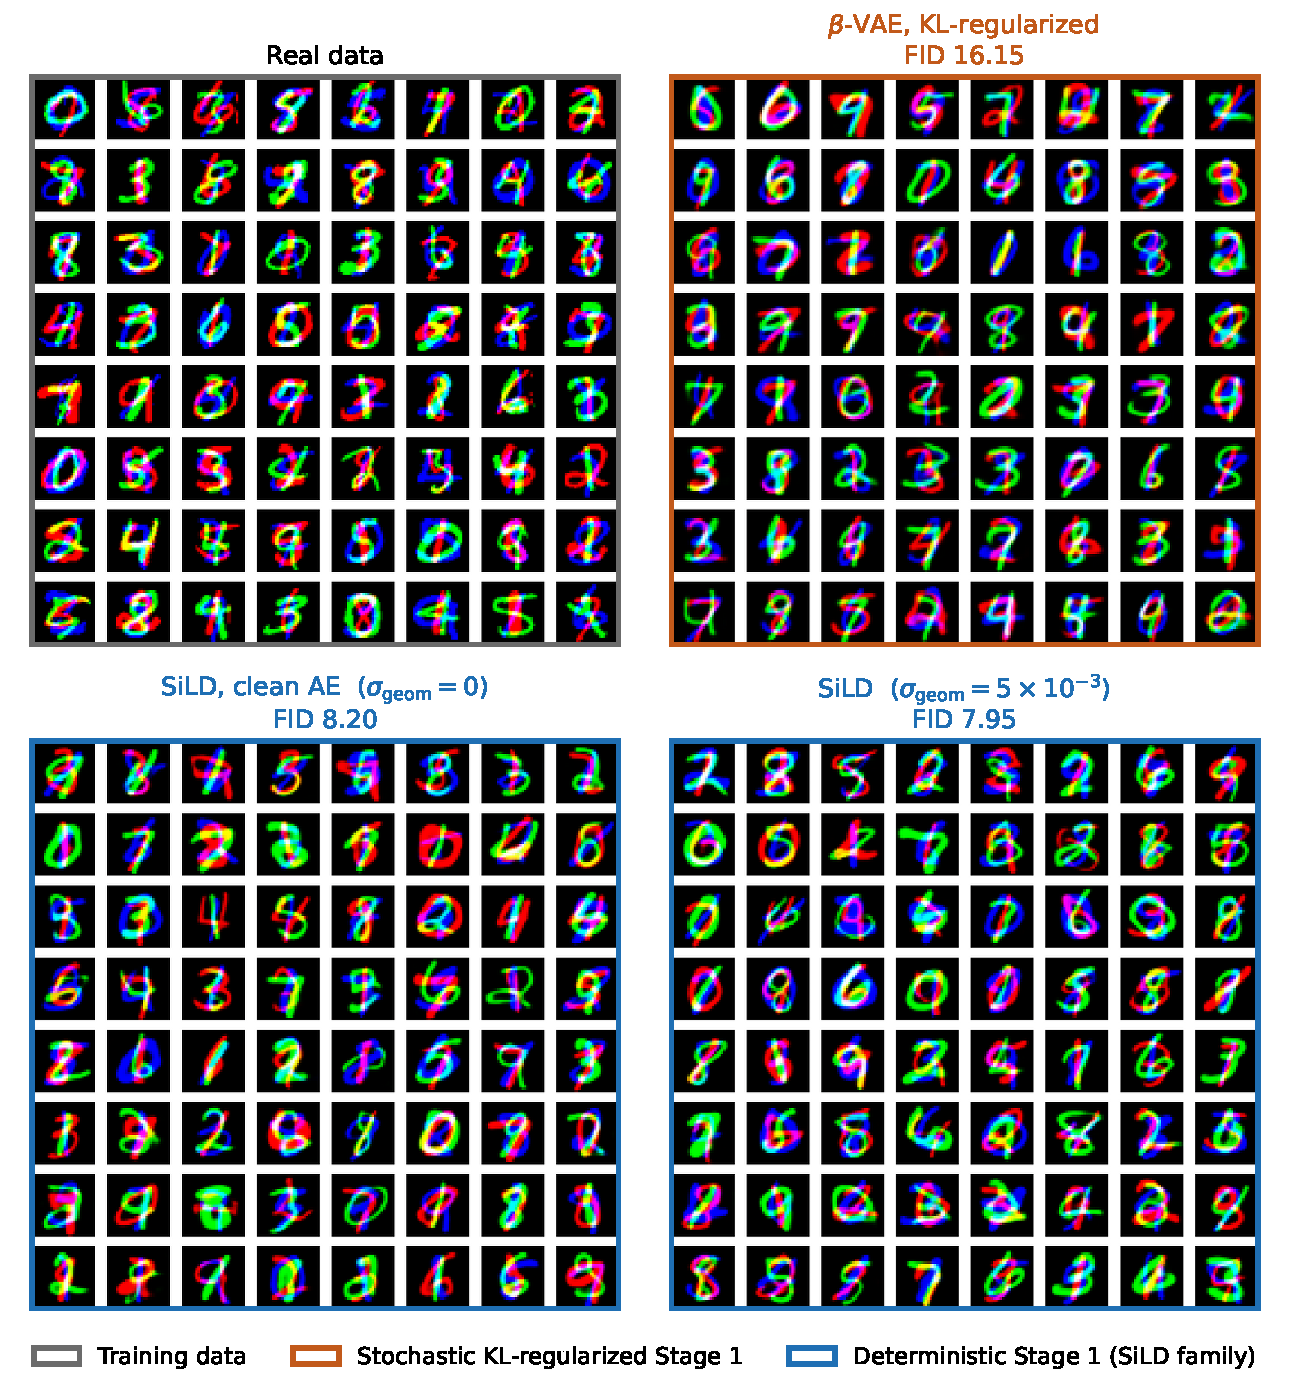
\includegraphics[width=\textwidth]{figures/stacked_mnist_stage1_family/stacked_mnist_stage1_family_seed42.pdf}
\caption{%
Uncurated Stacked MNIST samples for the three arms of
Table~\ref{tab:stacked_mnist}, plus real data (seed 42; each image is three
random MNIST digits stacked into the R/G/B channels, so there are 1000
possible modes). All panels come from runs that share the CNN backbones, the
latent score architecture, the training budget, and the Stage-2 interval
$t_2\in[0.001,0.999]$; only the Stage-1 objective differs. Every generative
arm attains full $1000/1000$ mode coverage, so none of the panels shows mode
dropping, and the qualitative differences are modest: the figure is included
to show that the clean autoencoder and SiLD are visually interchangeable
while both differ from the KL-regularized arm, which is the claim
Table~\ref{tab:stage1_noise_sweep} makes quantitatively. The remaining arms
of that table are omitted here; in particular the VP-schedule row is a
noise-form check rather than a noise-scale point and would not sit on the
same axis as the panels shown. FID values are repeated from
Table~\ref{tab:stage1_noise_sweep}.%
}
\label{fig:stacked_family_samples}
\end{figure}

\subsection{The Stage-1 objective family on molecules}
\label{app:stage1-family-mol}

Table~\ref{tab:stage1_family_mol} repeats the comparison of
Appendix~\ref{app:stage1-noise} on the molecular benchmarks. The degenerate
$\sigma\!\to\!0$ member of the family --- a clean deterministic autoencoder ---
matches SiLD on all four datasets to within $0.43$ FCD and $0.19$ percentage
points of uniqueness, with the sign of the difference inconsistent across
datasets and metrics. Each molecular cell is a single seed, so we do not
claim an ordering between the two deterministic arms; on Stacked MNIST, where
we do have three seeds, the corresponding paired difference is not
significant ($t=-0.96$). Both deterministic arms are separated from the
KL-regularized bottleneck by two orders of magnitude of uniqueness on HIV and
PCBA, and SiLD's autoencoder reaches $4.2$--$8.8\times$ lower reconstruction
error than the KL-regularized one, with the largest factor on QM9, where the
two generative models are otherwise closest.

The Stage-1 noise scale is therefore not the active ingredient; the
determinism of the Stage-1 map is. This is what the analysis predicts rather
than a weakening of it: Stage~1 is charged with identifying the
tangent--normal split, and the small-noise regime is a plateau on which any
deterministic map whose bottleneck recovers the same subspace will serve.
What the analysis does exclude is an isotropic \emph{stochastic} bottleneck,
which injects variance in the normal directions that Stage~1 is supposed to
contract; Appendix~\ref{app:collapse} shows that this is exactly how the
KL-regularized arm fails.

\begin{table}[h]
\centering
\caption{%
The Stage-1 objective family on molecules, at a common Stage-2 interval
$t_2\in[0.001,0.999]$ for all three arms (10K samples, seed 42, SELFIES;
validity is $100\%$ throughout). Encoder, decoder, and latent score network
are identical across rows; only the Stage-1 objective differs.
$\sigma\!\to\!0$ denotes the degenerate member of the family: an ordinary
clean deterministic autoencoder, with no input corruption and no KL term.
This family comparison needs its own Stage-2 interval because the paired rule
$t_2\in[t_0,0.999]$ used in Table~\ref{tab:main_results} degenerates at
$t_0=0$, so all arms are instead fixed at $t_{\min}=0.001$; the SiLD and
KL-regularized numbers therefore differ in the third digit from
Table~\ref{tab:main_results}. Bold marks the numerically best value per
dataset and metric, but every cell is a single seed and the two deterministic
arms trade wins at a margin we do not treat as meaningful.%
}
\label{tab:stage1_family_mol}
\resizebox{\textwidth}{!}{%
\begin{tabular}{llcccccc}
\toprule
\textbf{Dataset} & \textbf{Stage-1 objective}
& \textbf{Recon MSE$\downarrow$} & \textbf{Uniq.$\uparrow$}
& \textbf{Novelty$\uparrow$} & \textbf{Int.\ Div.$\uparrow$}
& \textbf{QED$\uparrow$} & \textbf{FCD$\downarrow$} \\
\midrule
\multirow{4}{*}{\textbf{QM9}}
 & Real data                               & --                      & 96.18\% & 0.0\%   & 0.919 & 0.466 & 5.05 \\
\cmidrule{2-8}
 & $\beta$-VAE, KL-regularized (LDM)       & $1.31\!\times\!10^{-3}$ & 96.94\% & 37.59\% & 0.915 & 0.473 & \textbf{4.30} \\
 & \textbf{SiLD} ($\sigma\!\to\!0$; clean AE) & $1.63\!\times\!10^{-4}$ & 97.43\% & 34.94\% & 0.917 & 0.471 & 4.41 \\
 & \textbf{SiLD} ($t_0=0.05$)              & $\mathbf{1.49\!\times\!10^{-4}}$ & \textbf{97.58\%} & 36.25\% & 0.917 & 0.468 & 4.39 \\
\midrule
\multirow{4}{*}{\textbf{HIV}}
 & Real data                               & --                      & 88.93\% & 0.0\%   & 0.898 & 0.513 & 3.24 \\
\cmidrule{2-8}
 & $\beta$-VAE, KL-regularized (LDM)       & $1.39\!\times\!10^{-3}$ & 0.99\%  & 100.0\% & 0.012 & 0.114 & 60.96 \\
 & \textbf{SiLD} ($\sigma\!\to\!0$; clean AE) & $3.28\!\times\!10^{-4}$ & \textbf{98.82\%} & 99.95\% & 0.904 & 0.430 & \textbf{10.29} \\
 & \textbf{SiLD} ($t_0=0.05$)              & $\mathbf{3.24\!\times\!10^{-4}}$ & 98.63\% & 99.95\% & 0.903 & 0.434 & 10.44 \\
\midrule
\multirow{4}{*}{\textbf{MUV}}
 & Real data                               & --                      & 95.03\% & 0.0\%   & 0.860 & 0.675 & 4.52 \\
\cmidrule{2-8}
 & $\beta$-VAE, KL-regularized (LDM)       & $6.55\!\times\!10^{-3}$ & 95.30\% & 99.98\% & 0.812 & 0.238 & 41.20 \\
 & \textbf{SiLD} ($\sigma\!\to\!0$; clean AE) & $1.60\!\times\!10^{-3}$ & \textbf{99.45\%} & 99.96\% & 0.892 & 0.513 & 19.85 \\
 & \textbf{SiLD} ($t_0=0.05$)              & $\mathbf{1.55\!\times\!10^{-3}}$ & 99.42\% & 99.97\% & 0.891 & 0.512 & \textbf{19.42} \\
\midrule
\multirow{4}{*}{\textbf{PCBA}}
 & Real data                               & --                      & 98.91\% & 0.0\%   & 0.861 & 0.637 & 9.12 \\
\cmidrule{2-8}
 & $\beta$-VAE, KL-regularized (LDM)       & $2.34\!\times\!10^{-3}$ & 0.57\%  & 94.74\% & 0.016 & 0.090 & 77.10 \\
 & \textbf{SiLD} ($\sigma\!\to\!0$; clean AE) & $5.41\!\times\!10^{-4}$ & \textbf{98.81\%} & 99.76\% & 0.895 & 0.483 & 18.04 \\
 & \textbf{SiLD} ($t_0=0.05$)              & $\mathbf{5.33\!\times\!10^{-4}}$ & 98.63\% & 99.78\% & 0.894 & 0.486 & \textbf{17.96} \\
\bottomrule
\end{tabular}%
}
\end{table}

\subsection{Stage-2 lower time bound}
\label{app:stage2-tmin}

Table~\ref{tab:stage2_tmin} varies the Stage-2 lower time bound on the
molecular benchmarks. This ablation does \emph{not} retrain Stage~1: a single
Stage-1 checkpoint (trained at $t_0=0.05$) is reused in every row, and only
the Stage-2 score network is retrained with the stated lower bound. It
therefore isolates the Stage-2 time range, not the Stage-1 noise scale, for
which Appendix~\ref{app:stage1-noise} is the relevant experiment. FCD varies
by at most $1.34$ (MUV) and by less than $0.16$ on QM9 and HIV.

\begin{table}[h]
\centering
\caption{%
Stage-2 lower time bound $t_{\min}$ on the molecular benchmarks, with Stage~1
held fixed at a single checkpoint trained at $t_0=0.05$. 10K samples, 200
sampling steps, seed 42.%
}
\label{tab:stage2_tmin}
\small
\begin{tabular}{lcccccccc}
\toprule
& \multicolumn{2}{c}{\textbf{QM9}} & \multicolumn{2}{c}{\textbf{HIV}}
& \multicolumn{2}{c}{\textbf{MUV}} & \multicolumn{2}{c}{\textbf{PCBA}} \\
\cmidrule(lr){2-3}\cmidrule(lr){4-5}\cmidrule(lr){6-7}\cmidrule(lr){8-9}
$t_{\min}$ & Uniq. & FCD & Uniq. & FCD & Uniq. & FCD & Uniq. & FCD \\
\midrule
$0.01$ & 97.44\% & 4.32 & 98.81\% & 10.35 & 99.35\% & 19.14 & 98.64\% & 17.95 \\
$0.02$ & 97.69\% & 4.47 & 98.76\% & 10.34 & 99.35\% & 19.23 & 98.70\% & 17.89 \\
$0.05$ & 97.23\% & 4.43 & 98.68\% & 10.32 & 99.31\% & 19.35 & 98.65\% & 17.87 \\
$0.10$ & 97.21\% & 4.33 & 98.65\% & 10.51 & 99.48\% & 18.86 & 98.93\% & 17.67 \\
$0.20$ & 97.29\% & 4.44 & 98.86\% & 10.44 & 99.38\% & 18.14 & 98.94\% & 17.08 \\
\bottomrule
\end{tabular}
\end{table}

\subsection{Where the KL-regularized arm fails}
\label{app:collapse}

To locate the failure we decompose the pipeline into three decodes that share
one trained model: \textbf{(A)} \emph{round trip} --- encode real test
molecules and decode, which exercises Stage~1 alone; \textbf{(B)}
\emph{generation} --- the full reverse latent diffusion followed by decoding;
and \textbf{(C)} \emph{prior decode} --- decode samples from
$\mathcal N(0,I)$ directly, bypassing the score network. If a model's
diversity were destroyed by the latent diffusion, (A) would be healthy and
(B) degraded. Table~\ref{tab:collapse_abc} shows the opposite for the
KL-regularized arm: (A) is already collapsed, and (A), (B), and (C) agree,
so the decoder's output is nearly independent of its input.

\begin{table}[h]
\centering
\caption{%
Pipeline decomposition, 10K samples per cell, seed 42. (A) encode real
molecules and decode; (B) full latent-diffusion generation; (C) decode
$\mathcal N(0,I)$ samples directly. For the KL-regularized arm on HIV and
PCBA all three agree at near-zero uniqueness and IntDiv, identifying Stage~1
as the point of failure.%
}
\label{tab:collapse_abc}
\small
\resizebox{\textwidth}{!}{%
\begin{tabular}{llccccccc}
\toprule
& & \multicolumn{3}{c}{\textbf{(A) round trip}} & \multicolumn{2}{c}{\textbf{(B) generation}} & \multicolumn{2}{c}{\textbf{(C) prior decode}} \\
\cmidrule(lr){3-5}\cmidrule(lr){6-7}\cmidrule(lr){8-9}
\textbf{Dataset} & \textbf{Stage-1 objective} & Uniq. & Int.\ Div. & FCD & Uniq. & FCD & Uniq. & FCD \\
\midrule
\multirow{2}{*}{\textbf{QM9}}
 & $\beta$-VAE, KL-regularized & 100.0\% & 0.917 & 6.09 & 99.61\% & 4.72 & 100.0\% & 5.72 \\
 & \textbf{SiLD}               & 100.0\% & 0.919 & 5.94 & 100.0\% & 5.10 & 98.05\% & 8.68 \\
\midrule
\multirow{2}{*}{\textbf{HIV}}
 & $\beta$-VAE, KL-regularized & 0.95\%  & 0.019 & 60.95 & 0.98\%  & 60.91 & 0.93\%  & 61.17 \\
 & \textbf{SiLD}               & 87.76\% & 0.902 & 5.09  & 98.84\% & 10.40 & 93.97\% & 17.67 \\
\midrule
\multirow{2}{*}{\textbf{PCBA}}
 & $\beta$-VAE, KL-regularized & 0.53\%  & 0.020 & 77.10 & 0.58\%  & 77.12 & 0.65\%  & 77.06 \\
 & \textbf{SiLD}               & 97.79\% & 0.885 & 11.03 & 98.72\% & 18.04 & 92.13\% & 28.63 \\
\bottomrule
\end{tabular}%
}
\end{table}

Table~\ref{tab:collapse_latent} gives the mechanism. On the raw encoder
output, the KL-regularized arm has driven $99.6\%$ (HIV) and $92.6\%$ (PCBA)
of coordinates to standard deviation below $10^{-3}$, with a
largest-to-smallest ratio in the thousands; SiLD has no such coordinate and a
ratio below $5$. On QM9 --- the one dataset where the two methods are
comparable --- the KL arm has no collapsed coordinates either, which is
consistent with the claim that posterior collapse, not KL regularization per
se, is what the two-stage separation avoids. The effective ranks in the last
three columns are computed after per-coordinate standardization, so they
measure the dimension of the occupied support rather than collapse; in every
arm the generated support matches the real support closely, while the
Gaussian prior occupies a far larger subspace.

\begin{table}[h]
\centering
\caption{%
Latent statistics, 10K encodings, seed 42. Dead coordinates and the
standard-deviation ratio (largest over smallest, and ``dead'' meaning
standard deviation below $10^{-3}$) are computed on the \emph{raw} encoder
output; effective rank (participation ratio) is computed after
per-coordinate standardization, on real encodings ($z_{\mathrm{real}}$), on
latents produced by Stage~2 ($z_{\mathrm{gen}}$), and on prior samples
($z_{\mathrm{prior}}$).%
}
\label{tab:collapse_latent}
\small
\resizebox{\textwidth}{!}{%
\begin{tabular}{llcccccc}
\toprule
\textbf{Dataset} & \textbf{Stage-1 objective} & $d_z$
& dead coords & std ratio
& eff.\ rank $z_{\mathrm{real}}$ & eff.\ rank $z_{\mathrm{gen}}$
& eff.\ rank $z_{\mathrm{prior}}$ \\
\midrule
\multirow{2}{*}{\textbf{QM9}}
 & $\beta$-VAE, KL-regularized & 128 & 0.0\%   & 80.4   & 3.10  & 3.42  & 84.9 \\
 & \textbf{SiLD}               & 128 & 0.0\%   & 2.0    & 25.08 & 26.84 & 85.8 \\
\midrule
\multirow{2}{*}{\textbf{HIV}}
 & $\beta$-VAE, KL-regularized & 512 & 99.6\%  & 2739.2 & 17.84 & 11.43 & 453.6 \\
 & \textbf{SiLD}               & 512 & 0.0\%   & 4.6    & 8.68  & 8.07  & 454.1 \\
\midrule
\multirow{2}{*}{\textbf{PCBA}}
 & $\beta$-VAE, KL-regularized & 256 & 92.6\%  & 1753.5 & 16.86 & 16.12 & 240.6 \\
 & \textbf{SiLD}               & 256 & 0.0\%   & 3.5    & 7.91  & 7.73  & 240.4 \\
\bottomrule
\end{tabular}%
}
\end{table}

In the SiLD latents the generated and real supports agree in effective rank
(participation ratio $8.07$ vs.\ $8.68$ out of $512$ on HIV, $7.73$ vs.\
$7.91$ out of $256$ on PCBA) while the Gaussian prior occupies $454$ and
$240$ respectively, so Stage~2 reproduces a support of the same low dimension
as the data rather than filling the latent cube.
Appendix~\ref{app:celeba-boundary} marks where the
deterministic-versus-KL ordering stops holding.

\subsection{Sampling-step budget}
\label{app:steps}

Table~\ref{tab:steps_sweep} varies the number of reverse-diffusion steps at
sampling time with the trained model held fixed. Quality is essentially flat
from $25$ to $500$ steps on all four molecular benchmarks: the FCD spread is
$0.30$ (QM9), $0.35$ (HIV), $0.97$ (MUV), and $0.68$ (PCBA), and the cheapest
setting is not systematically the worst. Generating 10K molecules takes
$1.3$--$1.7$\,s at $25$ steps against $21.6$--$22.3$\,s at $500$.

\begin{table}[h]
\centering
\caption{%
Reverse-diffusion step count at sampling time, with the trained SiLD model
held fixed. 10K samples, seed 42; wall-clock is the sampling time for the
full 10K batch on one GPU.%
}
\label{tab:steps_sweep}
\small
\begin{tabular}{lcccccccccc}
\toprule
& \multicolumn{2}{c}{\textbf{QM9}} & \multicolumn{2}{c}{\textbf{HIV}}
& \multicolumn{2}{c}{\textbf{MUV}} & \multicolumn{2}{c}{\textbf{PCBA}}
& \multicolumn{2}{c}{\textbf{wall-clock (s)}} \\
\cmidrule(lr){2-3}\cmidrule(lr){4-5}\cmidrule(lr){6-7}\cmidrule(lr){8-9}\cmidrule(lr){10-11}
steps & Uniq. & FCD & Uniq. & FCD & Uniq. & FCD & Uniq. & FCD & min & max \\
\midrule
$25$  & 97.44\% & 4.14 & 98.58\% & 10.81 & 99.53\% & 20.30 & 98.47\% & 18.44 & 1.3 & 1.7 \\
$50$  & 97.77\% & 4.27 & 98.69\% & 10.51 & 99.41\% & 19.73 & 98.59\% & 17.94 & 2.2 & 2.6 \\
$100$ & 97.36\% & 4.22 & 98.79\% & 10.49 & 99.24\% & 19.52 & 98.76\% & 17.76 & 4.3 & 4.8 \\
$200$ & 97.65\% & 4.38 & 98.78\% & 10.46 & 99.33\% & 19.33 & 98.67\% & 17.83 & 8.7 & 9.1 \\
$500$ & 97.73\% & 4.44 & 98.77\% & 10.49 & 99.44\% & 19.50 & 98.74\% & 17.99 & 21.6 & 22.3 \\
\bottomrule
\end{tabular}
\end{table}

\subsection{Novelty--fidelity trade-off on QM9}
\label{app:novelty-tradeoff}

QM9 is the one benchmark on which SiLD does not improve novelty over the
KL-regularized baseline (Table~\ref{tab:main_results}). The dataset is small
and nearly exhaustively enumerated, so novelty and distributional fidelity
are in direct tension there, and both are reachable from the same trained
model by rescaling the initial latent noise or the score at sampling time.
Table~\ref{tab:novelty_tradeoff} traces that frontier: inflating the initial
noise from $\sigma_{\mathrm{init}}=1.0$ to $1.3$ raises novelty from $35.8\%$
to $51.7\%$ and uniqueness from $97.5\%$ to $98.4\%$ while FCD degrades only
from $4.22$ to $5.19$; pushing further, or raising the score temperature,
buys novelty up to $97.7\%$ at a clear cost in FCD and QED. We report the
untuned $\sigma_{\mathrm{init}}=1.0$ setting everywhere in the main text.

\begin{table}[h]
\centering
\caption{%
Sampling-time novelty--fidelity trade-off on QM9, from a single trained SiLD
model (10K samples, 50 steps, seed 42). $\sigma_{\mathrm{init}}$ scales the
initial latent noise; $T$ scales the predicted score. The first row is the
setting used in the main text.%
}
\label{tab:novelty_tradeoff}
\small
\begin{tabular}{llccccc}
\toprule
$\sigma_{\mathrm{init}}$ & $T$ & Uniq.$\uparrow$ & Novelty$\uparrow$ & Int.\ Div.$\uparrow$ & QED$\uparrow$ & FCD$\downarrow$ \\
\midrule
$1.0$ & $1.0$ & 97.51\% & 35.8\% & 0.917 & 0.470 & 4.22 \\
$1.1$ & $1.0$ & 97.91\% & 42.0\% & 0.921 & 0.465 & 4.56 \\
$1.2$ & $1.0$ & 98.12\% & 46.5\% & 0.924 & 0.461 & 4.99 \\
$1.3$ & $1.0$ & 98.44\% & 51.7\% & 0.925 & 0.457 & 5.19 \\
$1.5$ & $1.0$ & 98.50\% & 61.3\% & 0.930 & 0.448 & 5.90 \\
$2.0$ & $1.0$ & 97.87\% & 80.7\% & 0.937 & 0.419 & 6.66 \\
\midrule
$1.0$ & $1.1$ & 98.47\% & 62.0\% & 0.928 & 0.448 & 5.43 \\
$1.0$ & $1.2$ & 97.76\% & 82.8\% & 0.937 & 0.418 & 6.20 \\
$1.0$ & $1.3$ & 91.45\% & 94.6\% & 0.944 & 0.366 & 7.94 \\
$1.0$ & $1.5$ & 86.37\% & 97.7\% & 0.946 & 0.324 & 9.61 \\
\midrule
$1.2$ & $1.2$ & 94.61\% & 91.8\% & 0.942 & 0.388 & 7.19 \\
$1.3$ & $1.2$ & 91.49\% & 94.4\% & 0.943 & 0.370 & 7.87 \\
$1.5$ & $1.3$ & 87.02\% & 97.8\% & 0.947 & 0.324 & 9.77 \\
\bottomrule
\end{tabular}
\end{table}

\subsection{Boundary of the deterministic-versus-KL ordering}
\label{app:celeba-boundary}

The ordering between deterministic and KL-regularized Stage-1 objectives is
not universal, and Table~\ref{tab:celeba_boundary} marks where it reverses.
On CelebA at $64\times64$ with a small KL weight ($10^{-4}$) and no auxiliary
regularizer, the KL-regularized arm attains the best FID and the best
reconstruction, and the pure deterministic autoencoder is worst. The latent
MMD to a standard Gaussian explains the reversal: the KL term is doing its
intended job of matching the prior ($0.0078$ against $0.0150$ for both
deterministic arms), and on this dataset it does so without collapsing any
coordinate --- exactly the regime in which Appendix~\ref{app:collapse}
predicts that removing KL buys nothing. Recovering the ordering on CelebA
requires an auxiliary prior-matching term in place of KL, which is what the
MMD- and GAN-regularized variants in the main text supply.

\begin{table}[h]
\centering
\caption{%
CelebA ($64\times64$), seed 42, identical encoder, decoder, and score network;
FID on 2048 samples, 500 sampling steps, $20$K Stage-1 and $60$K Stage-2
steps. ``Latent MMD'' is the maximum mean discrepancy between the encoded
data and $\mathcal N(0,I)$. No auxiliary regularizer (MMD, GAN, LPIPS) is
active in any row.%
}
\label{tab:celeba_boundary}
\small
\begin{tabular}{lcccc}
\toprule
Stage-1 objective & Recon MSE $\downarrow$ & Latent MMD $\downarrow$ & $\epsilon$-loss $\downarrow$ & FID $\downarrow$ \\
\midrule
$\beta$-VAE, KL-regularized ($\lambda_{\mathrm{KL}}=10^{-4}$) & $\mathbf{1.283\!\times\!10^{-3}}$ & $\mathbf{0.0078}$ & $\mathbf{0.277}$ & $\mathbf{63.64}$ \\
SiLD ($\sigma_{\mathrm{geom}}=5\!\times\!10^{-3}$)            & $1.338\!\times\!10^{-3}$ & $0.0150$ & $0.315$ & $64.70$ \\
SiLD, clean AE ($\sigma_{\mathrm{geom}}=0$)                   & $1.449\!\times\!10^{-3}$ & $0.0151$ & $0.318$ & $66.06$ \\
\bottomrule
\end{tabular}
\end{table}

% ---------------------------------------------------------------------
% OPEN ITEM: the subsection below reports a result that is unfavourable to
% SiLD. It is drafted so it is ready to use, but whether to include it is a
% judgement call that has not been made yet. Delete the subsection if not.
% ---------------------------------------------------------------------
\subsection{Equivariant 3D molecular latents: a negative result}
\label{app:3d}

The two-stage separation does not help when the latent already carries a
strong geometric inductive bias. Substituting the SiLD Stage-1 objective into
the E(3)-equivariant autoencoder of GeoLDM~\cite{xu2023geometric} on QM9 with
3D coordinates, and training both arms identically, leaves SiLD behind the
KL-regularized original on every stability and validity metric
(Table~\ref{tab:qm9_3d}). We report this rather than omitting it: the
mechanism identified in Appendix~\ref{app:collapse} is posterior collapse in
a generic bottleneck, and an equivariant encoder whose latent is tied to
atom-wise geometry does not exhibit it, so the premise for the improvement is
absent. Both arms also remain far below the published GeoLDM numbers under
our reduced training budget, so the comparison should be read as a matched
ablation and not as a reproduction.

\begin{table}[h]
\centering
\caption{%
QM9 with 3D coordinates, E(3)-equivariant GeoLDM backbone, 10K samples.
Both arms in the upper block come from one paired run with identical
budgets; the last row is a separately trained KL-regularized arm. Atom and
molecule stability follow the standard valency-based definitions.%
}
\label{tab:qm9_3d}
\small
\begin{tabular}{lcccc}
\toprule
Stage-1 objective & Atom stab.$\uparrow$ & Mol.\ stab.$\uparrow$ & Validity$\uparrow$ & Valid \& unique$\uparrow$ \\
\midrule
Real data                                & 95.13\% & 93.92\% & 95.28\% & 91.55\% \\
\midrule
$\beta$-VAE, KL-regularized (GeoLDM)     & \textbf{45.80\%} & \textbf{38.09\%} & \textbf{47.52\%} & \textbf{47.41\%} \\
SiLD Stage-1 in the GeoLDM latent        & 42.94\% & 32.89\% & 44.65\% & 44.61\% \\
\midrule
$\beta$-VAE, KL-regularized (separate run) & 49.11\% & 45.14\% & 50.20\% & 49.88\% \\
\bottomrule
\end{tabular}
\end{table}

% Cross-referenced from the main text via app:stage1-noise and app:collapse.

\section{Additional experimental results}
\label{app:extra-experiments}

\subsection{Stage-1 noise scale}
\label{app:stage1-noise}

Table~\ref{tab:stage1_noise_sweep} sweeps the Stage-1 corruption scale on
Stacked MNIST with everything else held fixed: each arm trains its own
Stage-1 map at the stated $\sigma_{\mathrm{geom}}$ and its own Stage-2 score
network on the common interval $t_2\in[0.001,0.999]$, at three seeds (42, 43,
44). Across the three additive noise levels, FID moves by $0.25$ with no
monotone trend, and the paired per-seed differences against the
$\sigma_{\mathrm{geom}}=0$ arm are not significant at either level
($\lvert t\rvert \le 0.96$, $n=3$), with the sign flipping across seeds. The
KL-regularized arm differs from all of them by $8$ FID and by a factor $1.8$
in reconstruction error. The Stage-1 noise scale is thus a plateau, and the
deterministic-versus-stochastic distinction is the one that carries the
effect. Figure~\ref{fig:stacked_family_samples} shows the corresponding
uncurated samples.

The last row of Table~\ref{tab:stage1_noise_sweep} is a separate check and
not a fourth point on the $\sigma_{\mathrm{geom}}$ axis. For the Stacked
MNIST experiments we replace the VP corruption of
Algorithm~\ref{alg:practical-sild} by additive constant-$\sigma$ corruption;
that row restores the VP form at the same nominal $t_0=5\!\times\!10^{-3}$,
which induces an effective standard deviation of $2.74\!\times\!10^{-2}$,
$5.5\times$ larger than the additive arm at the same $t_0$. It therefore
varies the noise \emph{form} and its \emph{magnitude} at once, and we report
it only to confirm that the substitution is immaterial: FID
$8.271 \pm 0.031$, paired $t=+0.74$ against $\sigma_{\mathrm{geom}}=0$.

\begin{table}[h]
\centering
\caption{%
Stacked MNIST Stage-1 noise sweep. Every arm is separately trained and uses
the same CNN backbones, latent score architecture, training budget, and
Stage-2 interval $t_2\in[0.001,0.999]$. Mean$\pm$population std over seeds
42, 43, 44; FID on 10K samples, mode coverage on 25{,}600 samples. The last
column is the per-seed paired FID difference against the
$\sigma_{\mathrm{geom}}=0$ arm (negative favours the row). The upper block
varies the additive Stage-1 noise scale; the last row instead restores the VP
corruption of Algorithm~\ref{alg:practical-sild} at the same nominal
$t_0=5\!\times\!10^{-3}$, which induces the larger effective
$\sigma_{\mathrm{geom}}$ shown, so it varies the noise form and magnitude
together and is not comparable to the rows above as a noise-scale point.%
}
\label{tab:stage1_noise_sweep}
\small
\begin{tabular}{lccccc}
\toprule
Stage-1 objective & $\sigma_{\mathrm{geom}}$ & \#modes & Recon MSE ($\times10^{-3}$) $\downarrow$ & FID $\downarrow$ & $\Delta$FID vs.\ $\sigma\!=\!0$ \\
\midrule
$\beta$-VAE, KL-reg.\ (LDM-CNN)      & ---                   & 1000 & $6.284 \pm 0.052$ & $16.152 \pm 0.098$ & --- \\
\midrule
SiLD, clean AE ($\sigma\!\to\!0$)    & $0$                   & 1000 & $3.542 \pm 0.036$ & $8.199 \pm 0.137$  & (reference) \\
SiLD                                 & $1\!\times\!10^{-3}$  & 1000 & $3.533 \pm 0.014$ & $8.187 \pm 0.102$  & $-0.012$ ($t=-0.14$) \\
SiLD                                 & $5\!\times\!10^{-3}$  & 1000 & $3.539 \pm 0.017$ & $7.951 \pm 0.262$  & $-0.248$ ($t=-0.96$) \\
\midrule
\multicolumn{6}{l}{\emph{Noise form (parameterization check, not a point on the $\sigma_{\mathrm{geom}}$ axis)}} \\
SiLD, VP schedule at $t_0\!=\!5\!\times\!10^{-3}$ & $2.74\!\times\!10^{-2}$ (induced) & 1000 & $3.561 \pm 0.026$ & $8.271 \pm 0.031$  & $+0.072$ ($t=+0.74$) \\
\bottomrule
\end{tabular}
\end{table}

\begin{figure}[h]
\centering
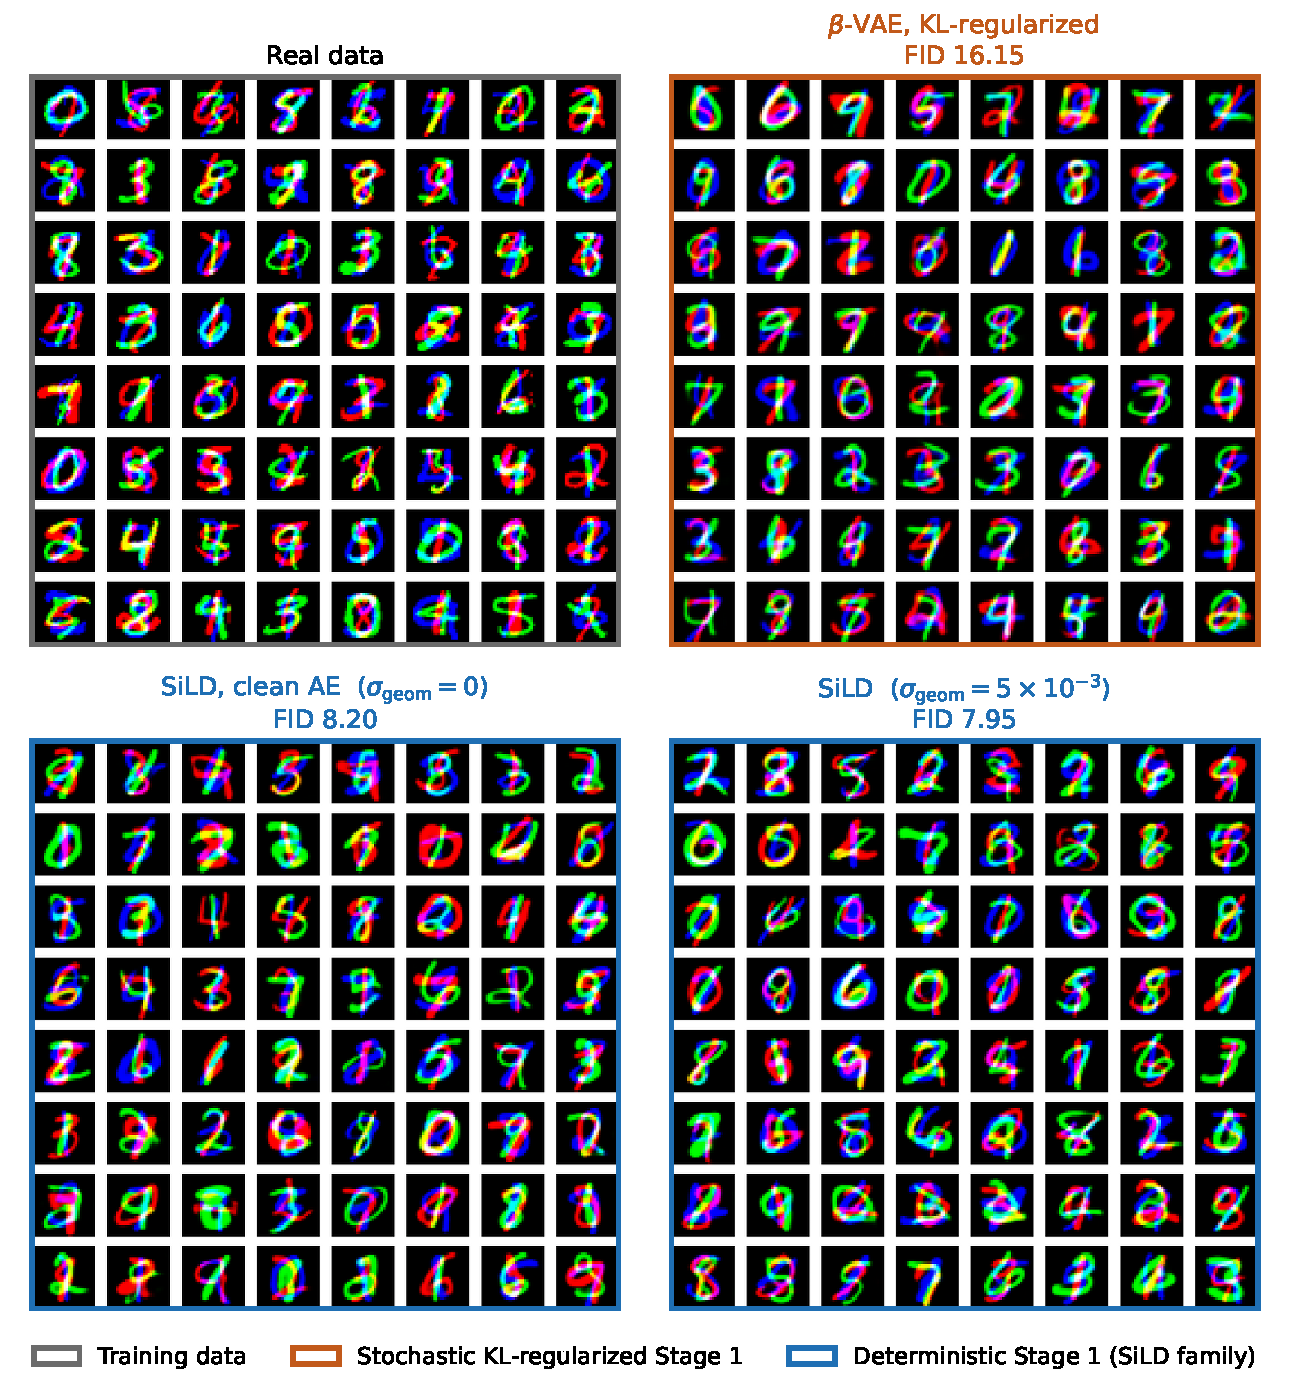
\includegraphics[width=\textwidth]{figures/stacked_mnist_stage1_family/stacked_mnist_stage1_family_seed42.pdf}
\caption{%
Uncurated Stacked MNIST samples for the three arms of
Table~\ref{tab:stacked_mnist}, plus real data (seed 42; each image is three
random MNIST digits stacked into the R/G/B channels, so there are 1000
possible modes). All panels come from runs that share the CNN backbones, the
latent score architecture, the training budget, and the Stage-2 interval
$t_2\in[0.001,0.999]$; only the Stage-1 objective differs. Every generative
arm attains full $1000/1000$ mode coverage, so none of the panels shows mode
dropping, and the qualitative differences are modest: the figure is included
to show that the clean autoencoder and SiLD are visually interchangeable
while both differ from the KL-regularized arm, which is the claim
Table~\ref{tab:stage1_noise_sweep} makes quantitatively. The remaining arms
of that table are omitted here; in particular the VP-schedule row is a
noise-form check rather than a noise-scale point and would not sit on the
same axis as the panels shown. FID values are repeated from
Table~\ref{tab:stage1_noise_sweep}.%
}
\label{fig:stacked_family_samples}
\end{figure}

\subsection{The Stage-1 objective family on molecules}
\label{app:stage1-family-mol}

Table~\ref{tab:stage1_family_mol} repeats the comparison of
Appendix~\ref{app:stage1-noise} on the molecular benchmarks. The degenerate
$\sigma\!\to\!0$ member of the family --- a clean deterministic autoencoder ---
matches SiLD on all four datasets to within $0.43$ FCD and $0.19$ percentage
points of uniqueness, with the sign of the difference inconsistent across
datasets and metrics. Each molecular cell is a single seed, so we do not
claim an ordering between the two deterministic arms; on Stacked MNIST, where
we do have three seeds, the corresponding paired difference is not
significant ($t=-0.96$). Both deterministic arms are separated from the
KL-regularized bottleneck by two orders of magnitude of uniqueness on HIV and
PCBA, and SiLD's autoencoder reaches $4.2$--$8.8\times$ lower reconstruction
error than the KL-regularized one, with the largest factor on QM9, where the
two generative models are otherwise closest.

The Stage-1 noise scale is therefore not the active ingredient; the
determinism of the Stage-1 map is. This is what the analysis predicts rather
than a weakening of it: Stage~1 is charged with identifying the
tangent--normal split, and the small-noise regime is a plateau on which any
deterministic map whose bottleneck recovers the same subspace will serve.
What the analysis does exclude is an isotropic \emph{stochastic} bottleneck,
which injects variance in the normal directions that Stage~1 is supposed to
contract; Appendix~\ref{app:collapse} shows that this is exactly how the
KL-regularized arm fails.

\begin{table}[h]
\centering
\caption{%
The Stage-1 objective family on molecules, at a common Stage-2 interval
$t_2\in[0.001,0.999]$ for all three arms (10K samples, seed 42, SELFIES;
validity is $100\%$ throughout). Encoder, decoder, and latent score network
are identical across rows; only the Stage-1 objective differs.
$\sigma\!\to\!0$ denotes the degenerate member of the family: an ordinary
clean deterministic autoencoder, with no input corruption and no KL term.
This family comparison needs its own Stage-2 interval because the paired rule
$t_2\in[t_0,0.999]$ used in Table~\ref{tab:main_results} degenerates at
$t_0=0$, so all arms are instead fixed at $t_{\min}=0.001$; the SiLD and
KL-regularized numbers therefore differ in the third digit from
Table~\ref{tab:main_results}. Bold marks the numerically best value per
dataset and metric, but every cell is a single seed and the two deterministic
arms trade wins at a margin we do not treat as meaningful.%
}
\label{tab:stage1_family_mol}
\resizebox{\textwidth}{!}{%
\begin{tabular}{llcccccc}
\toprule
\textbf{Dataset} & \textbf{Stage-1 objective}
& \textbf{Recon MSE$\downarrow$} & \textbf{Uniq.$\uparrow$}
& \textbf{Novelty$\uparrow$} & \textbf{Int.\ Div.$\uparrow$}
& \textbf{QED$\uparrow$} & \textbf{FCD$\downarrow$} \\
\midrule
\multirow{4}{*}{\textbf{QM9}}
 & Real data                               & --                      & 96.18\% & 0.0\%   & 0.919 & 0.466 & 5.05 \\
\cmidrule{2-8}
 & $\beta$-VAE, KL-regularized (LDM)       & $1.31\!\times\!10^{-3}$ & 96.94\% & 37.59\% & 0.915 & 0.473 & \textbf{4.30} \\
 & \textbf{SiLD} ($\sigma\!\to\!0$; clean AE) & $1.63\!\times\!10^{-4}$ & 97.43\% & 34.94\% & 0.917 & 0.471 & 4.41 \\
 & \textbf{SiLD} ($t_0=0.05$)              & $\mathbf{1.49\!\times\!10^{-4}}$ & \textbf{97.58\%} & 36.25\% & 0.917 & 0.468 & 4.39 \\
\midrule
\multirow{4}{*}{\textbf{HIV}}
 & Real data                               & --                      & 88.93\% & 0.0\%   & 0.898 & 0.513 & 3.24 \\
\cmidrule{2-8}
 & $\beta$-VAE, KL-regularized (LDM)       & $1.39\!\times\!10^{-3}$ & 0.99\%  & 100.0\% & 0.012 & 0.114 & 60.96 \\
 & \textbf{SiLD} ($\sigma\!\to\!0$; clean AE) & $3.28\!\times\!10^{-4}$ & \textbf{98.82\%} & 99.95\% & 0.904 & 0.430 & \textbf{10.29} \\
 & \textbf{SiLD} ($t_0=0.05$)              & $\mathbf{3.24\!\times\!10^{-4}}$ & 98.63\% & 99.95\% & 0.903 & 0.434 & 10.44 \\
\midrule
\multirow{4}{*}{\textbf{MUV}}
 & Real data                               & --                      & 95.03\% & 0.0\%   & 0.860 & 0.675 & 4.52 \\
\cmidrule{2-8}
 & $\beta$-VAE, KL-regularized (LDM)       & $6.55\!\times\!10^{-3}$ & 95.30\% & 99.98\% & 0.812 & 0.238 & 41.20 \\
 & \textbf{SiLD} ($\sigma\!\to\!0$; clean AE) & $1.60\!\times\!10^{-3}$ & \textbf{99.45\%} & 99.96\% & 0.892 & 0.513 & 19.85 \\
 & \textbf{SiLD} ($t_0=0.05$)              & $\mathbf{1.55\!\times\!10^{-3}}$ & 99.42\% & 99.97\% & 0.891 & 0.512 & \textbf{19.42} \\
\midrule
\multirow{4}{*}{\textbf{PCBA}}
 & Real data                               & --                      & 98.91\% & 0.0\%   & 0.861 & 0.637 & 9.12 \\
\cmidrule{2-8}
 & $\beta$-VAE, KL-regularized (LDM)       & $2.34\!\times\!10^{-3}$ & 0.57\%  & 94.74\% & 0.016 & 0.090 & 77.10 \\
 & \textbf{SiLD} ($\sigma\!\to\!0$; clean AE) & $5.41\!\times\!10^{-4}$ & \textbf{98.81\%} & 99.76\% & 0.895 & 0.483 & 18.04 \\
 & \textbf{SiLD} ($t_0=0.05$)              & $\mathbf{5.33\!\times\!10^{-4}}$ & 98.63\% & 99.78\% & 0.894 & 0.486 & \textbf{17.96} \\
\bottomrule
\end{tabular}%
}
\end{table}

\subsection{Stage-2 lower time bound}
\label{app:stage2-tmin}

Table~\ref{tab:stage2_tmin} varies the Stage-2 lower time bound on the
molecular benchmarks. This ablation does \emph{not} retrain Stage~1: a single
Stage-1 checkpoint (trained at $t_0=0.05$) is reused in every row, and only
the Stage-2 score network is retrained with the stated lower bound. It
therefore isolates the Stage-2 time range, not the Stage-1 noise scale, for
which Appendix~\ref{app:stage1-noise} is the relevant experiment. FCD varies
by at most $1.34$ (MUV) and by less than $0.16$ on QM9 and HIV.

\begin{table}[h]
\centering
\caption{%
Stage-2 lower time bound $t_{\min}$ on the molecular benchmarks, with Stage~1
held fixed at a single checkpoint trained at $t_0=0.05$. 10K samples, 200
sampling steps, seed 42.%
}
\label{tab:stage2_tmin}
\small
\begin{tabular}{lcccccccc}
\toprule
& \multicolumn{2}{c}{\textbf{QM9}} & \multicolumn{2}{c}{\textbf{HIV}}
& \multicolumn{2}{c}{\textbf{MUV}} & \multicolumn{2}{c}{\textbf{PCBA}} \\
\cmidrule(lr){2-3}\cmidrule(lr){4-5}\cmidrule(lr){6-7}\cmidrule(lr){8-9}
$t_{\min}$ & Uniq. & FCD & Uniq. & FCD & Uniq. & FCD & Uniq. & FCD \\
\midrule
$0.01$ & 97.44\% & 4.32 & 98.81\% & 10.35 & 99.35\% & 19.14 & 98.64\% & 17.95 \\
$0.02$ & 97.69\% & 4.47 & 98.76\% & 10.34 & 99.35\% & 19.23 & 98.70\% & 17.89 \\
$0.05$ & 97.23\% & 4.43 & 98.68\% & 10.32 & 99.31\% & 19.35 & 98.65\% & 17.87 \\
$0.10$ & 97.21\% & 4.33 & 98.65\% & 10.51 & 99.48\% & 18.86 & 98.93\% & 17.67 \\
$0.20$ & 97.29\% & 4.44 & 98.86\% & 10.44 & 99.38\% & 18.14 & 98.94\% & 17.08 \\
\bottomrule
\end{tabular}
\end{table}

\subsection{Where the KL-regularized arm fails}
\label{app:collapse}

To locate the failure we decompose the pipeline into three decodes that share
one trained model: \textbf{(A)} \emph{round trip} --- encode real test
molecules and decode, which exercises Stage~1 alone; \textbf{(B)}
\emph{generation} --- the full reverse latent diffusion followed by decoding;
and \textbf{(C)} \emph{prior decode} --- decode samples from
$\mathcal N(0,I)$ directly, bypassing the score network. If a model's
diversity were destroyed by the latent diffusion, (A) would be healthy and
(B) degraded. Table~\ref{tab:collapse_abc} shows the opposite for the
KL-regularized arm: (A) is already collapsed, and (A), (B), and (C) agree,
so the decoder's output is nearly independent of its input.

\begin{table}[h]
\centering
\caption{%
Pipeline decomposition, 10K samples per cell, seed 42. (A) encode real
molecules and decode; (B) full latent-diffusion generation; (C) decode
$\mathcal N(0,I)$ samples directly. For the KL-regularized arm on HIV and
PCBA all three agree at near-zero uniqueness and IntDiv, identifying Stage~1
as the point of failure.%
}
\label{tab:collapse_abc}
\small
\resizebox{\textwidth}{!}{%
\begin{tabular}{llccccccc}
\toprule
& & \multicolumn{3}{c}{\textbf{(A) round trip}} & \multicolumn{2}{c}{\textbf{(B) generation}} & \multicolumn{2}{c}{\textbf{(C) prior decode}} \\
\cmidrule(lr){3-5}\cmidrule(lr){6-7}\cmidrule(lr){8-9}
\textbf{Dataset} & \textbf{Stage-1 objective} & Uniq. & Int.\ Div. & FCD & Uniq. & FCD & Uniq. & FCD \\
\midrule
\multirow{2}{*}{\textbf{QM9}}
 & $\beta$-VAE, KL-regularized & 100.0\% & 0.917 & 6.09 & 99.61\% & 4.72 & 100.0\% & 5.72 \\
 & \textbf{SiLD}               & 100.0\% & 0.919 & 5.94 & 100.0\% & 5.10 & 98.05\% & 8.68 \\
\midrule
\multirow{2}{*}{\textbf{HIV}}
 & $\beta$-VAE, KL-regularized & 0.95\%  & 0.019 & 60.95 & 0.98\%  & 60.91 & 0.93\%  & 61.17 \\
 & \textbf{SiLD}               & 87.76\% & 0.902 & 5.09  & 98.84\% & 10.40 & 93.97\% & 17.67 \\
\midrule
\multirow{2}{*}{\textbf{PCBA}}
 & $\beta$-VAE, KL-regularized & 0.53\%  & 0.020 & 77.10 & 0.58\%  & 77.12 & 0.65\%  & 77.06 \\
 & \textbf{SiLD}               & 97.79\% & 0.885 & 11.03 & 98.72\% & 18.04 & 92.13\% & 28.63 \\
\bottomrule
\end{tabular}%
}
\end{table}

Table~\ref{tab:collapse_latent} gives the mechanism. On the raw encoder
output, the KL-regularized arm has driven $99.6\%$ (HIV) and $92.6\%$ (PCBA)
of coordinates to standard deviation below $10^{-3}$, with a
largest-to-smallest ratio in the thousands; SiLD has no such coordinate and a
ratio below $5$. On QM9 --- the one dataset where the two methods are
comparable --- the KL arm has no collapsed coordinates either, which is
consistent with the claim that posterior collapse, not KL regularization per
se, is what the two-stage separation avoids. The effective ranks in the last
three columns are computed after per-coordinate standardization, so they
measure the dimension of the occupied support rather than collapse; in every
arm the generated support matches the real support closely, while the
Gaussian prior occupies a far larger subspace.

\begin{table}[h]
\centering
\caption{%
Latent statistics, 10K encodings, seed 42. Dead coordinates and the
standard-deviation ratio (largest over smallest, and ``dead'' meaning
standard deviation below $10^{-3}$) are computed on the \emph{raw} encoder
output; effective rank (participation ratio) is computed after
per-coordinate standardization, on real encodings ($z_{\mathrm{real}}$), on
latents produced by Stage~2 ($z_{\mathrm{gen}}$), and on prior samples
($z_{\mathrm{prior}}$).%
}
\label{tab:collapse_latent}
\small
\resizebox{\textwidth}{!}{%
\begin{tabular}{llcccccc}
\toprule
\textbf{Dataset} & \textbf{Stage-1 objective} & $d_z$
& dead coords & std ratio
& eff.\ rank $z_{\mathrm{real}}$ & eff.\ rank $z_{\mathrm{gen}}$
& eff.\ rank $z_{\mathrm{prior}}$ \\
\midrule
\multirow{2}{*}{\textbf{QM9}}
 & $\beta$-VAE, KL-regularized & 128 & 0.0\%   & 80.4   & 3.10  & 3.42  & 84.9 \\
 & \textbf{SiLD}               & 128 & 0.0\%   & 2.0    & 25.08 & 26.84 & 85.8 \\
\midrule
\multirow{2}{*}{\textbf{HIV}}
 & $\beta$-VAE, KL-regularized & 512 & 99.6\%  & 2739.2 & 17.84 & 11.43 & 453.6 \\
 & \textbf{SiLD}               & 512 & 0.0\%   & 4.6    & 8.68  & 8.07  & 454.1 \\
\midrule
\multirow{2}{*}{\textbf{PCBA}}
 & $\beta$-VAE, KL-regularized & 256 & 92.6\%  & 1753.5 & 16.86 & 16.12 & 240.6 \\
 & \textbf{SiLD}               & 256 & 0.0\%   & 3.5    & 7.91  & 7.73  & 240.4 \\
\bottomrule
\end{tabular}%
}
\end{table}

In the SiLD latents the generated and real supports agree in effective rank
(participation ratio $8.07$ vs.\ $8.68$ out of $512$ on HIV, $7.73$ vs.\
$7.91$ out of $256$ on PCBA) while the Gaussian prior occupies $454$ and
$240$ respectively, so Stage~2 reproduces a support of the same low dimension
as the data rather than filling the latent cube.
Appendix~\ref{app:celeba-boundary} marks where the
deterministic-versus-KL ordering stops holding.

\subsection{Sampling-step budget}
\label{app:steps}

Table~\ref{tab:steps_sweep} varies the number of reverse-diffusion steps at
sampling time with the trained model held fixed. Quality is essentially flat
from $25$ to $500$ steps on all four molecular benchmarks: the FCD spread is
$0.30$ (QM9), $0.35$ (HIV), $0.97$ (MUV), and $0.68$ (PCBA), and the cheapest
setting is not systematically the worst. Generating 10K molecules takes
$1.3$--$1.7$\,s at $25$ steps against $21.6$--$22.3$\,s at $500$.

\begin{table}[h]
\centering
\caption{%
Reverse-diffusion step count at sampling time, with the trained SiLD model
held fixed. 10K samples, seed 42; wall-clock is the sampling time for the
full 10K batch on one GPU.%
}
\label{tab:steps_sweep}
\small
\begin{tabular}{lcccccccccc}
\toprule
& \multicolumn{2}{c}{\textbf{QM9}} & \multicolumn{2}{c}{\textbf{HIV}}
& \multicolumn{2}{c}{\textbf{MUV}} & \multicolumn{2}{c}{\textbf{PCBA}}
& \multicolumn{2}{c}{\textbf{wall-clock (s)}} \\
\cmidrule(lr){2-3}\cmidrule(lr){4-5}\cmidrule(lr){6-7}\cmidrule(lr){8-9}\cmidrule(lr){10-11}
steps & Uniq. & FCD & Uniq. & FCD & Uniq. & FCD & Uniq. & FCD & min & max \\
\midrule
$25$  & 97.44\% & 4.14 & 98.58\% & 10.81 & 99.53\% & 20.30 & 98.47\% & 18.44 & 1.3 & 1.7 \\
$50$  & 97.77\% & 4.27 & 98.69\% & 10.51 & 99.41\% & 19.73 & 98.59\% & 17.94 & 2.2 & 2.6 \\
$100$ & 97.36\% & 4.22 & 98.79\% & 10.49 & 99.24\% & 19.52 & 98.76\% & 17.76 & 4.3 & 4.8 \\
$200$ & 97.65\% & 4.38 & 98.78\% & 10.46 & 99.33\% & 19.33 & 98.67\% & 17.83 & 8.7 & 9.1 \\
$500$ & 97.73\% & 4.44 & 98.77\% & 10.49 & 99.44\% & 19.50 & 98.74\% & 17.99 & 21.6 & 22.3 \\
\bottomrule
\end{tabular}
\end{table}

\subsection{Novelty--fidelity trade-off on QM9}
\label{app:novelty-tradeoff}

QM9 is the one benchmark on which SiLD does not improve novelty over the
KL-regularized baseline (Table~\ref{tab:main_results}). The dataset is small
and nearly exhaustively enumerated, so novelty and distributional fidelity
are in direct tension there, and both are reachable from the same trained
model by rescaling the initial latent noise or the score at sampling time.
Table~\ref{tab:novelty_tradeoff} traces that frontier: inflating the initial
noise from $\sigma_{\mathrm{init}}=1.0$ to $1.3$ raises novelty from $35.8\%$
to $51.7\%$ and uniqueness from $97.5\%$ to $98.4\%$ while FCD degrades only
from $4.22$ to $5.19$; pushing further, or raising the score temperature,
buys novelty up to $97.7\%$ at a clear cost in FCD and QED. We report the
untuned $\sigma_{\mathrm{init}}=1.0$ setting everywhere in the main text.

\begin{table}[h]
\centering
\caption{%
Sampling-time novelty--fidelity trade-off on QM9, from a single trained SiLD
model (10K samples, 50 steps, seed 42). $\sigma_{\mathrm{init}}$ scales the
initial latent noise; $T$ scales the predicted score. The first row is the
setting used in the main text.%
}
\label{tab:novelty_tradeoff}
\small
\begin{tabular}{llccccc}
\toprule
$\sigma_{\mathrm{init}}$ & $T$ & Uniq.$\uparrow$ & Novelty$\uparrow$ & Int.\ Div.$\uparrow$ & QED$\uparrow$ & FCD$\downarrow$ \\
\midrule
$1.0$ & $1.0$ & 97.51\% & 35.8\% & 0.917 & 0.470 & 4.22 \\
$1.1$ & $1.0$ & 97.91\% & 42.0\% & 0.921 & 0.465 & 4.56 \\
$1.2$ & $1.0$ & 98.12\% & 46.5\% & 0.924 & 0.461 & 4.99 \\
$1.3$ & $1.0$ & 98.44\% & 51.7\% & 0.925 & 0.457 & 5.19 \\
$1.5$ & $1.0$ & 98.50\% & 61.3\% & 0.930 & 0.448 & 5.90 \\
$2.0$ & $1.0$ & 97.87\% & 80.7\% & 0.937 & 0.419 & 6.66 \\
\midrule
$1.0$ & $1.1$ & 98.47\% & 62.0\% & 0.928 & 0.448 & 5.43 \\
$1.0$ & $1.2$ & 97.76\% & 82.8\% & 0.937 & 0.418 & 6.20 \\
$1.0$ & $1.3$ & 91.45\% & 94.6\% & 0.944 & 0.366 & 7.94 \\
$1.0$ & $1.5$ & 86.37\% & 97.7\% & 0.946 & 0.324 & 9.61 \\
\midrule
$1.2$ & $1.2$ & 94.61\% & 91.8\% & 0.942 & 0.388 & 7.19 \\
$1.3$ & $1.2$ & 91.49\% & 94.4\% & 0.943 & 0.370 & 7.87 \\
$1.5$ & $1.3$ & 87.02\% & 97.8\% & 0.947 & 0.324 & 9.77 \\
\bottomrule
\end{tabular}
\end{table}

\subsection{Boundary of the deterministic-versus-KL ordering}
\label{app:celeba-boundary}

The ordering between deterministic and KL-regularized Stage-1 objectives is
not universal, and Table~\ref{tab:celeba_boundary} marks where it reverses.
On CelebA at $64\times64$ with a small KL weight ($10^{-4}$) and no auxiliary
regularizer, the KL-regularized arm attains the best FID and the best
reconstruction, and the pure deterministic autoencoder is worst. The latent
MMD to a standard Gaussian explains the reversal: the KL term is doing its
intended job of matching the prior ($0.0078$ against $0.0150$ for both
deterministic arms), and on this dataset it does so without collapsing any
coordinate --- exactly the regime in which Appendix~\ref{app:collapse}
predicts that removing KL buys nothing. Recovering the ordering on CelebA
requires an auxiliary prior-matching term in place of KL, which is what the
MMD- and GAN-regularized variants in the main text supply.

\begin{table}[h]
\centering
\caption{%
CelebA ($64\times64$), seed 42, identical encoder, decoder, and score network;
FID on 2048 samples, 500 sampling steps, $20$K Stage-1 and $60$K Stage-2
steps. ``Latent MMD'' is the maximum mean discrepancy between the encoded
data and $\mathcal N(0,I)$. No auxiliary regularizer (MMD, GAN, LPIPS) is
active in any row.%
}
\label{tab:celeba_boundary}
\small
\begin{tabular}{lcccc}
\toprule
Stage-1 objective & Recon MSE $\downarrow$ & Latent MMD $\downarrow$ & $\epsilon$-loss $\downarrow$ & FID $\downarrow$ \\
\midrule
$\beta$-VAE, KL-regularized ($\lambda_{\mathrm{KL}}=10^{-4}$) & $\mathbf{1.283\!\times\!10^{-3}}$ & $\mathbf{0.0078}$ & $\mathbf{0.277}$ & $\mathbf{63.64}$ \\
SiLD ($\sigma_{\mathrm{geom}}=5\!\times\!10^{-3}$)            & $1.338\!\times\!10^{-3}$ & $0.0150$ & $0.315$ & $64.70$ \\
SiLD, clean AE ($\sigma_{\mathrm{geom}}=0$)                   & $1.449\!\times\!10^{-3}$ & $0.0151$ & $0.318$ & $66.06$ \\
\bottomrule
\end{tabular}
\end{table}

% ---------------------------------------------------------------------
% OPEN ITEM: the subsection below reports a result that is unfavourable to
% SiLD. It is drafted so it is ready to use, but whether to include it is a
% judgement call that has not been made yet. Delete the subsection if not.
% ---------------------------------------------------------------------
\subsection{Equivariant 3D molecular latents: a negative result}
\label{app:3d}

The two-stage separation does not help when the latent already carries a
strong geometric inductive bias. Substituting the SiLD Stage-1 objective into
the E(3)-equivariant autoencoder of GeoLDM~\cite{xu2023geometric} on QM9 with
3D coordinates, and training both arms identically, leaves SiLD behind the
KL-regularized original on every stability and validity metric
(Table~\ref{tab:qm9_3d}). We report this rather than omitting it: the
mechanism identified in Appendix~\ref{app:collapse} is posterior collapse in
a generic bottleneck, and an equivariant encoder whose latent is tied to
atom-wise geometry does not exhibit it, so the premise for the improvement is
absent. Both arms also remain far below the published GeoLDM numbers under
our reduced training budget, so the comparison should be read as a matched
ablation and not as a reproduction.

\begin{table}[h]
\centering
\caption{%
QM9 with 3D coordinates, E(3)-equivariant GeoLDM backbone, 10K samples.
Both arms in the upper block come from one paired run with identical
budgets; the last row is a separately trained KL-regularized arm. Atom and
molecule stability follow the standard valency-based definitions.%
}
\label{tab:qm9_3d}
\small
\begin{tabular}{lcccc}
\toprule
Stage-1 objective & Atom stab.$\uparrow$ & Mol.\ stab.$\uparrow$ & Validity$\uparrow$ & Valid \& unique$\uparrow$ \\
\midrule
Real data                                & 95.13\% & 93.92\% & 95.28\% & 91.55\% \\
\midrule
$\beta$-VAE, KL-regularized (GeoLDM)     & \textbf{45.80\%} & \textbf{38.09\%} & \textbf{47.52\%} & \textbf{47.41\%} \\
SiLD Stage-1 in the GeoLDM latent        & 42.94\% & 32.89\% & 44.65\% & 44.61\% \\
\midrule
$\beta$-VAE, KL-regularized (separate run) & 49.11\% & 45.14\% & 50.20\% & 49.88\% \\
\bottomrule
\end{tabular}
\end{table}

% Cross-referenced from the main text via app:stage1-noise and app:collapse.

\section{Additional experimental results}
\label{app:extra-experiments}

\subsection{Stage-1 noise scale}
\label{app:stage1-noise}

Table~\ref{tab:stage1_noise_sweep} sweeps the Stage-1 corruption scale on
Stacked MNIST with everything else held fixed: each arm trains its own
Stage-1 map at the stated $\sigma_{\mathrm{geom}}$ and its own Stage-2 score
network on the common interval $t_2\in[0.001,0.999]$, at three seeds (42, 43,
44). Across the three additive noise levels, FID moves by $0.25$ with no
monotone trend, and the paired per-seed differences against the
$\sigma_{\mathrm{geom}}=0$ arm are not significant at either level
($\lvert t\rvert \le 0.96$, $n=3$), with the sign flipping across seeds. The
KL-regularized arm differs from all of them by $8$ FID and by a factor $1.8$
in reconstruction error. The Stage-1 noise scale is thus a plateau, and the
deterministic-versus-stochastic distinction is the one that carries the
effect. Figure~\ref{fig:stacked_family_samples} shows the corresponding
uncurated samples.

The last row of Table~\ref{tab:stage1_noise_sweep} is a separate check and
not a fourth point on the $\sigma_{\mathrm{geom}}$ axis. For the Stacked
MNIST experiments we replace the VP corruption of
Algorithm~\ref{alg:practical-sild} by additive constant-$\sigma$ corruption;
that row restores the VP form at the same nominal $t_0=5\!\times\!10^{-3}$,
which induces an effective standard deviation of $2.74\!\times\!10^{-2}$,
$5.5\times$ larger than the additive arm at the same $t_0$. It therefore
varies the noise \emph{form} and its \emph{magnitude} at once, and we report
it only to confirm that the substitution is immaterial: FID
$8.271 \pm 0.031$, paired $t=+0.74$ against $\sigma_{\mathrm{geom}}=0$.

\begin{table}[h]
\centering
\caption{%
Stacked MNIST Stage-1 noise sweep. Every arm is separately trained and uses
the same CNN backbones, latent score architecture, training budget, and
Stage-2 interval $t_2\in[0.001,0.999]$. Mean$\pm$population std over seeds
42, 43, 44; FID on 10K samples, mode coverage on 25{,}600 samples. The last
column is the per-seed paired FID difference against the
$\sigma_{\mathrm{geom}}=0$ arm (negative favours the row). The upper block
varies the additive Stage-1 noise scale; the last row instead restores the VP
corruption of Algorithm~\ref{alg:practical-sild} at the same nominal
$t_0=5\!\times\!10^{-3}$, which induces the larger effective
$\sigma_{\mathrm{geom}}$ shown, so it varies the noise form and magnitude
together and is not comparable to the rows above as a noise-scale point.%
}
\label{tab:stage1_noise_sweep}
\small
\begin{tabular}{lccccc}
\toprule
Stage-1 objective & $\sigma_{\mathrm{geom}}$ & \#modes & Recon MSE ($\times10^{-3}$) $\downarrow$ & FID $\downarrow$ & $\Delta$FID vs.\ $\sigma\!=\!0$ \\
\midrule
$\beta$-VAE, KL-reg.\ (LDM-CNN)      & ---                   & 1000 & $6.284 \pm 0.052$ & $16.152 \pm 0.098$ & --- \\
\midrule
SiLD, clean AE ($\sigma\!\to\!0$)    & $0$                   & 1000 & $3.542 \pm 0.036$ & $8.199 \pm 0.137$  & (reference) \\
SiLD                                 & $1\!\times\!10^{-3}$  & 1000 & $3.533 \pm 0.014$ & $8.187 \pm 0.102$  & $-0.012$ ($t=-0.14$) \\
SiLD                                 & $5\!\times\!10^{-3}$  & 1000 & $3.539 \pm 0.017$ & $7.951 \pm 0.262$  & $-0.248$ ($t=-0.96$) \\
\midrule
\multicolumn{6}{l}{\emph{Noise form (parameterization check, not a point on the $\sigma_{\mathrm{geom}}$ axis)}} \\
SiLD, VP schedule at $t_0\!=\!5\!\times\!10^{-3}$ & $2.74\!\times\!10^{-2}$ (induced) & 1000 & $3.561 \pm 0.026$ & $8.271 \pm 0.031$  & $+0.072$ ($t=+0.74$) \\
\bottomrule
\end{tabular}
\end{table}

\begin{figure}[h]
\centering
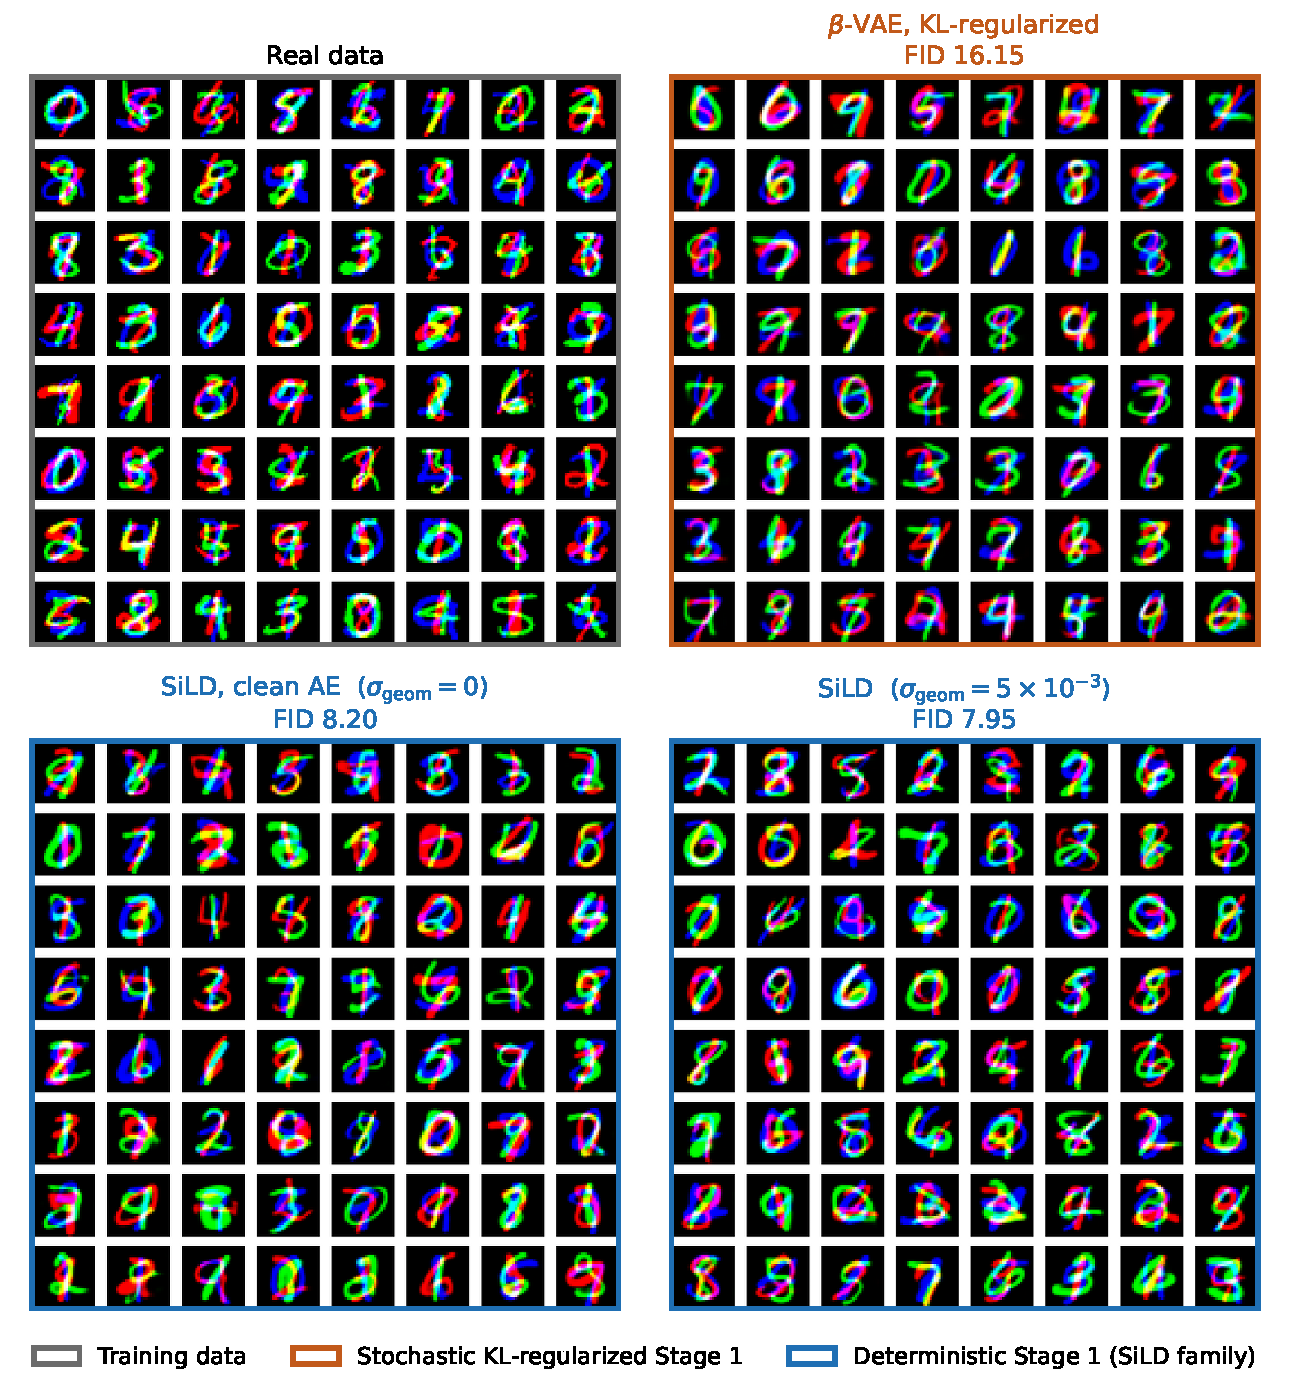
\includegraphics[width=\textwidth]{figures/stacked_mnist_stage1_family/stacked_mnist_stage1_family_seed42.pdf}
\caption{%
Uncurated Stacked MNIST samples for the three arms of
Table~\ref{tab:stacked_mnist}, plus real data (seed 42; each image is three
random MNIST digits stacked into the R/G/B channels, so there are 1000
possible modes). All panels come from runs that share the CNN backbones, the
latent score architecture, the training budget, and the Stage-2 interval
$t_2\in[0.001,0.999]$; only the Stage-1 objective differs. Every generative
arm attains full $1000/1000$ mode coverage, so none of the panels shows mode
dropping, and the qualitative differences are modest: the figure is included
to show that the clean autoencoder and SiLD are visually interchangeable
while both differ from the KL-regularized arm, which is the claim
Table~\ref{tab:stage1_noise_sweep} makes quantitatively. The remaining arms
of that table are omitted here; in particular the VP-schedule row is a
noise-form check rather than a noise-scale point and would not sit on the
same axis as the panels shown. FID values are repeated from
Table~\ref{tab:stage1_noise_sweep}.%
}
\label{fig:stacked_family_samples}
\end{figure}

\subsection{The Stage-1 objective family on molecules}
\label{app:stage1-family-mol}

Table~\ref{tab:stage1_family_mol} repeats the comparison of
Appendix~\ref{app:stage1-noise} on the molecular benchmarks. The degenerate
$\sigma\!\to\!0$ member of the family --- a clean deterministic autoencoder ---
matches SiLD on all four datasets to within $0.43$ FCD and $0.19$ percentage
points of uniqueness, with the sign of the difference inconsistent across
datasets and metrics. Each molecular cell is a single seed, so we do not
claim an ordering between the two deterministic arms; on Stacked MNIST, where
we do have three seeds, the corresponding paired difference is not
significant ($t=-0.96$). Both deterministic arms are separated from the
KL-regularized bottleneck by two orders of magnitude of uniqueness on HIV and
PCBA, and SiLD's autoencoder reaches $4.2$--$8.8\times$ lower reconstruction
error than the KL-regularized one, with the largest factor on QM9, where the
two generative models are otherwise closest.

The Stage-1 noise scale is therefore not the active ingredient; the
determinism of the Stage-1 map is. This is what the analysis predicts rather
than a weakening of it: Stage~1 is charged with identifying the
tangent--normal split, and the small-noise regime is a plateau on which any
deterministic map whose bottleneck recovers the same subspace will serve.
What the analysis does exclude is an isotropic \emph{stochastic} bottleneck,
which injects variance in the normal directions that Stage~1 is supposed to
contract; Appendix~\ref{app:collapse} shows that this is exactly how the
KL-regularized arm fails.

\begin{table}[h]
\centering
\caption{%
The Stage-1 objective family on molecules, at a common Stage-2 interval
$t_2\in[0.001,0.999]$ for all three arms (10K samples, seed 42, SELFIES;
validity is $100\%$ throughout). Encoder, decoder, and latent score network
are identical across rows; only the Stage-1 objective differs.
$\sigma\!\to\!0$ denotes the degenerate member of the family: an ordinary
clean deterministic autoencoder, with no input corruption and no KL term.
This family comparison needs its own Stage-2 interval because the paired rule
$t_2\in[t_0,0.999]$ used in Table~\ref{tab:main_results} degenerates at
$t_0=0$, so all arms are instead fixed at $t_{\min}=0.001$; the SiLD and
KL-regularized numbers therefore differ in the third digit from
Table~\ref{tab:main_results}. Bold marks the numerically best value per
dataset and metric, but every cell is a single seed and the two deterministic
arms trade wins at a margin we do not treat as meaningful.%
}
\label{tab:stage1_family_mol}
\resizebox{\textwidth}{!}{%
\begin{tabular}{llcccccc}
\toprule
\textbf{Dataset} & \textbf{Stage-1 objective}
& \textbf{Recon MSE$\downarrow$} & \textbf{Uniq.$\uparrow$}
& \textbf{Novelty$\uparrow$} & \textbf{Int.\ Div.$\uparrow$}
& \textbf{QED$\uparrow$} & \textbf{FCD$\downarrow$} \\
\midrule
\multirow{4}{*}{\textbf{QM9}}
 & Real data                               & --                      & 96.18\% & 0.0\%   & 0.919 & 0.466 & 5.05 \\
\cmidrule{2-8}
 & $\beta$-VAE, KL-regularized (LDM)       & $1.31\!\times\!10^{-3}$ & 96.94\% & 37.59\% & 0.915 & 0.473 & \textbf{4.30} \\
 & \textbf{SiLD} ($\sigma\!\to\!0$; clean AE) & $1.63\!\times\!10^{-4}$ & 97.43\% & 34.94\% & 0.917 & 0.471 & 4.41 \\
 & \textbf{SiLD} ($t_0=0.05$)              & $\mathbf{1.49\!\times\!10^{-4}}$ & \textbf{97.58\%} & 36.25\% & 0.917 & 0.468 & 4.39 \\
\midrule
\multirow{4}{*}{\textbf{HIV}}
 & Real data                               & --                      & 88.93\% & 0.0\%   & 0.898 & 0.513 & 3.24 \\
\cmidrule{2-8}
 & $\beta$-VAE, KL-regularized (LDM)       & $1.39\!\times\!10^{-3}$ & 0.99\%  & 100.0\% & 0.012 & 0.114 & 60.96 \\
 & \textbf{SiLD} ($\sigma\!\to\!0$; clean AE) & $3.28\!\times\!10^{-4}$ & \textbf{98.82\%} & 99.95\% & 0.904 & 0.430 & \textbf{10.29} \\
 & \textbf{SiLD} ($t_0=0.05$)              & $\mathbf{3.24\!\times\!10^{-4}}$ & 98.63\% & 99.95\% & 0.903 & 0.434 & 10.44 \\
\midrule
\multirow{4}{*}{\textbf{MUV}}
 & Real data                               & --                      & 95.03\% & 0.0\%   & 0.860 & 0.675 & 4.52 \\
\cmidrule{2-8}
 & $\beta$-VAE, KL-regularized (LDM)       & $6.55\!\times\!10^{-3}$ & 95.30\% & 99.98\% & 0.812 & 0.238 & 41.20 \\
 & \textbf{SiLD} ($\sigma\!\to\!0$; clean AE) & $1.60\!\times\!10^{-3}$ & \textbf{99.45\%} & 99.96\% & 0.892 & 0.513 & 19.85 \\
 & \textbf{SiLD} ($t_0=0.05$)              & $\mathbf{1.55\!\times\!10^{-3}}$ & 99.42\% & 99.97\% & 0.891 & 0.512 & \textbf{19.42} \\
\midrule
\multirow{4}{*}{\textbf{PCBA}}
 & Real data                               & --                      & 98.91\% & 0.0\%   & 0.861 & 0.637 & 9.12 \\
\cmidrule{2-8}
 & $\beta$-VAE, KL-regularized (LDM)       & $2.34\!\times\!10^{-3}$ & 0.57\%  & 94.74\% & 0.016 & 0.090 & 77.10 \\
 & \textbf{SiLD} ($\sigma\!\to\!0$; clean AE) & $5.41\!\times\!10^{-4}$ & \textbf{98.81\%} & 99.76\% & 0.895 & 0.483 & 18.04 \\
 & \textbf{SiLD} ($t_0=0.05$)              & $\mathbf{5.33\!\times\!10^{-4}}$ & 98.63\% & 99.78\% & 0.894 & 0.486 & \textbf{17.96} \\
\bottomrule
\end{tabular}%
}
\end{table}

\subsection{Stage-2 lower time bound}
\label{app:stage2-tmin}

Table~\ref{tab:stage2_tmin} varies the Stage-2 lower time bound on the
molecular benchmarks. This ablation does \emph{not} retrain Stage~1: a single
Stage-1 checkpoint (trained at $t_0=0.05$) is reused in every row, and only
the Stage-2 score network is retrained with the stated lower bound. It
therefore isolates the Stage-2 time range, not the Stage-1 noise scale, for
which Appendix~\ref{app:stage1-noise} is the relevant experiment. FCD varies
by at most $1.34$ (MUV) and by less than $0.16$ on QM9 and HIV.

\begin{table}[h]
\centering
\caption{%
Stage-2 lower time bound $t_{\min}$ on the molecular benchmarks, with Stage~1
held fixed at a single checkpoint trained at $t_0=0.05$. 10K samples, 200
sampling steps, seed 42.%
}
\label{tab:stage2_tmin}
\small
\begin{tabular}{lcccccccc}
\toprule
& \multicolumn{2}{c}{\textbf{QM9}} & \multicolumn{2}{c}{\textbf{HIV}}
& \multicolumn{2}{c}{\textbf{MUV}} & \multicolumn{2}{c}{\textbf{PCBA}} \\
\cmidrule(lr){2-3}\cmidrule(lr){4-5}\cmidrule(lr){6-7}\cmidrule(lr){8-9}
$t_{\min}$ & Uniq. & FCD & Uniq. & FCD & Uniq. & FCD & Uniq. & FCD \\
\midrule
$0.01$ & 97.44\% & 4.32 & 98.81\% & 10.35 & 99.35\% & 19.14 & 98.64\% & 17.95 \\
$0.02$ & 97.69\% & 4.47 & 98.76\% & 10.34 & 99.35\% & 19.23 & 98.70\% & 17.89 \\
$0.05$ & 97.23\% & 4.43 & 98.68\% & 10.32 & 99.31\% & 19.35 & 98.65\% & 17.87 \\
$0.10$ & 97.21\% & 4.33 & 98.65\% & 10.51 & 99.48\% & 18.86 & 98.93\% & 17.67 \\
$0.20$ & 97.29\% & 4.44 & 98.86\% & 10.44 & 99.38\% & 18.14 & 98.94\% & 17.08 \\
\bottomrule
\end{tabular}
\end{table}

\subsection{Where the KL-regularized arm fails}
\label{app:collapse}

To locate the failure we decompose the pipeline into three decodes that share
one trained model: \textbf{(A)} \emph{round trip} --- encode real test
molecules and decode, which exercises Stage~1 alone; \textbf{(B)}
\emph{generation} --- the full reverse latent diffusion followed by decoding;
and \textbf{(C)} \emph{prior decode} --- decode samples from
$\mathcal N(0,I)$ directly, bypassing the score network. If a model's
diversity were destroyed by the latent diffusion, (A) would be healthy and
(B) degraded. Table~\ref{tab:collapse_abc} shows the opposite for the
KL-regularized arm: (A) is already collapsed, and (A), (B), and (C) agree,
so the decoder's output is nearly independent of its input.

\begin{table}[h]
\centering
\caption{%
Pipeline decomposition, 10K samples per cell, seed 42. (A) encode real
molecules and decode; (B) full latent-diffusion generation; (C) decode
$\mathcal N(0,I)$ samples directly. For the KL-regularized arm on HIV and
PCBA all three agree at near-zero uniqueness and IntDiv, identifying Stage~1
as the point of failure.%
}
\label{tab:collapse_abc}
\small
\resizebox{\textwidth}{!}{%
\begin{tabular}{llccccccc}
\toprule
& & \multicolumn{3}{c}{\textbf{(A) round trip}} & \multicolumn{2}{c}{\textbf{(B) generation}} & \multicolumn{2}{c}{\textbf{(C) prior decode}} \\
\cmidrule(lr){3-5}\cmidrule(lr){6-7}\cmidrule(lr){8-9}
\textbf{Dataset} & \textbf{Stage-1 objective} & Uniq. & Int.\ Div. & FCD & Uniq. & FCD & Uniq. & FCD \\
\midrule
\multirow{2}{*}{\textbf{QM9}}
 & $\beta$-VAE, KL-regularized & 100.0\% & 0.917 & 6.09 & 99.61\% & 4.72 & 100.0\% & 5.72 \\
 & \textbf{SiLD}               & 100.0\% & 0.919 & 5.94 & 100.0\% & 5.10 & 98.05\% & 8.68 \\
\midrule
\multirow{2}{*}{\textbf{HIV}}
 & $\beta$-VAE, KL-regularized & 0.95\%  & 0.019 & 60.95 & 0.98\%  & 60.91 & 0.93\%  & 61.17 \\
 & \textbf{SiLD}               & 87.76\% & 0.902 & 5.09  & 98.84\% & 10.40 & 93.97\% & 17.67 \\
\midrule
\multirow{2}{*}{\textbf{PCBA}}
 & $\beta$-VAE, KL-regularized & 0.53\%  & 0.020 & 77.10 & 0.58\%  & 77.12 & 0.65\%  & 77.06 \\
 & \textbf{SiLD}               & 97.79\% & 0.885 & 11.03 & 98.72\% & 18.04 & 92.13\% & 28.63 \\
\bottomrule
\end{tabular}%
}
\end{table}

Table~\ref{tab:collapse_latent} gives the mechanism. On the raw encoder
output, the KL-regularized arm has driven $99.6\%$ (HIV) and $92.6\%$ (PCBA)
of coordinates to standard deviation below $10^{-3}$, with a
largest-to-smallest ratio in the thousands; SiLD has no such coordinate and a
ratio below $5$. On QM9 --- the one dataset where the two methods are
comparable --- the KL arm has no collapsed coordinates either, which is
consistent with the claim that posterior collapse, not KL regularization per
se, is what the two-stage separation avoids. The effective ranks in the last
three columns are computed after per-coordinate standardization, so they
measure the dimension of the occupied support rather than collapse; in every
arm the generated support matches the real support closely, while the
Gaussian prior occupies a far larger subspace.

\begin{table}[h]
\centering
\caption{%
Latent statistics, 10K encodings, seed 42. Dead coordinates and the
standard-deviation ratio (largest over smallest, and ``dead'' meaning
standard deviation below $10^{-3}$) are computed on the \emph{raw} encoder
output; effective rank (participation ratio) is computed after
per-coordinate standardization, on real encodings ($z_{\mathrm{real}}$), on
latents produced by Stage~2 ($z_{\mathrm{gen}}$), and on prior samples
($z_{\mathrm{prior}}$).%
}
\label{tab:collapse_latent}
\small
\resizebox{\textwidth}{!}{%
\begin{tabular}{llcccccc}
\toprule
\textbf{Dataset} & \textbf{Stage-1 objective} & $d_z$
& dead coords & std ratio
& eff.\ rank $z_{\mathrm{real}}$ & eff.\ rank $z_{\mathrm{gen}}$
& eff.\ rank $z_{\mathrm{prior}}$ \\
\midrule
\multirow{2}{*}{\textbf{QM9}}
 & $\beta$-VAE, KL-regularized & 128 & 0.0\%   & 80.4   & 3.10  & 3.42  & 84.9 \\
 & \textbf{SiLD}               & 128 & 0.0\%   & 2.0    & 25.08 & 26.84 & 85.8 \\
\midrule
\multirow{2}{*}{\textbf{HIV}}
 & $\beta$-VAE, KL-regularized & 512 & 99.6\%  & 2739.2 & 17.84 & 11.43 & 453.6 \\
 & \textbf{SiLD}               & 512 & 0.0\%   & 4.6    & 8.68  & 8.07  & 454.1 \\
\midrule
\multirow{2}{*}{\textbf{PCBA}}
 & $\beta$-VAE, KL-regularized & 256 & 92.6\%  & 1753.5 & 16.86 & 16.12 & 240.6 \\
 & \textbf{SiLD}               & 256 & 0.0\%   & 3.5    & 7.91  & 7.73  & 240.4 \\
\bottomrule
\end{tabular}%
}
\end{table}

In the SiLD latents the generated and real supports agree in effective rank
(participation ratio $8.07$ vs.\ $8.68$ out of $512$ on HIV, $7.73$ vs.\
$7.91$ out of $256$ on PCBA) while the Gaussian prior occupies $454$ and
$240$ respectively, so Stage~2 reproduces a support of the same low dimension
as the data rather than filling the latent cube.
Appendix~\ref{app:celeba-boundary} marks where the
deterministic-versus-KL ordering stops holding.

\subsection{Sampling-step budget}
\label{app:steps}

Table~\ref{tab:steps_sweep} varies the number of reverse-diffusion steps at
sampling time with the trained model held fixed. Quality is essentially flat
from $25$ to $500$ steps on all four molecular benchmarks: the FCD spread is
$0.30$ (QM9), $0.35$ (HIV), $0.97$ (MUV), and $0.68$ (PCBA), and the cheapest
setting is not systematically the worst. Generating 10K molecules takes
$1.3$--$1.7$\,s at $25$ steps against $21.6$--$22.3$\,s at $500$.

\begin{table}[h]
\centering
\caption{%
Reverse-diffusion step count at sampling time, with the trained SiLD model
held fixed. 10K samples, seed 42; wall-clock is the sampling time for the
full 10K batch on one GPU.%
}
\label{tab:steps_sweep}
\small
\begin{tabular}{lcccccccccc}
\toprule
& \multicolumn{2}{c}{\textbf{QM9}} & \multicolumn{2}{c}{\textbf{HIV}}
& \multicolumn{2}{c}{\textbf{MUV}} & \multicolumn{2}{c}{\textbf{PCBA}}
& \multicolumn{2}{c}{\textbf{wall-clock (s)}} \\
\cmidrule(lr){2-3}\cmidrule(lr){4-5}\cmidrule(lr){6-7}\cmidrule(lr){8-9}\cmidrule(lr){10-11}
steps & Uniq. & FCD & Uniq. & FCD & Uniq. & FCD & Uniq. & FCD & min & max \\
\midrule
$25$  & 97.44\% & 4.14 & 98.58\% & 10.81 & 99.53\% & 20.30 & 98.47\% & 18.44 & 1.3 & 1.7 \\
$50$  & 97.77\% & 4.27 & 98.69\% & 10.51 & 99.41\% & 19.73 & 98.59\% & 17.94 & 2.2 & 2.6 \\
$100$ & 97.36\% & 4.22 & 98.79\% & 10.49 & 99.24\% & 19.52 & 98.76\% & 17.76 & 4.3 & 4.8 \\
$200$ & 97.65\% & 4.38 & 98.78\% & 10.46 & 99.33\% & 19.33 & 98.67\% & 17.83 & 8.7 & 9.1 \\
$500$ & 97.73\% & 4.44 & 98.77\% & 10.49 & 99.44\% & 19.50 & 98.74\% & 17.99 & 21.6 & 22.3 \\
\bottomrule
\end{tabular}
\end{table}

\subsection{Novelty--fidelity trade-off on QM9}
\label{app:novelty-tradeoff}

QM9 is the one benchmark on which SiLD does not improve novelty over the
KL-regularized baseline (Table~\ref{tab:main_results}). The dataset is small
and nearly exhaustively enumerated, so novelty and distributional fidelity
are in direct tension there, and both are reachable from the same trained
model by rescaling the initial latent noise or the score at sampling time.
Table~\ref{tab:novelty_tradeoff} traces that frontier: inflating the initial
noise from $\sigma_{\mathrm{init}}=1.0$ to $1.3$ raises novelty from $35.8\%$
to $51.7\%$ and uniqueness from $97.5\%$ to $98.4\%$ while FCD degrades only
from $4.22$ to $5.19$; pushing further, or raising the score temperature,
buys novelty up to $97.7\%$ at a clear cost in FCD and QED. We report the
untuned $\sigma_{\mathrm{init}}=1.0$ setting everywhere in the main text.

\begin{table}[h]
\centering
\caption{%
Sampling-time novelty--fidelity trade-off on QM9, from a single trained SiLD
model (10K samples, 50 steps, seed 42). $\sigma_{\mathrm{init}}$ scales the
initial latent noise; $T$ scales the predicted score. The first row is the
setting used in the main text.%
}
\label{tab:novelty_tradeoff}
\small
\begin{tabular}{llccccc}
\toprule
$\sigma_{\mathrm{init}}$ & $T$ & Uniq.$\uparrow$ & Novelty$\uparrow$ & Int.\ Div.$\uparrow$ & QED$\uparrow$ & FCD$\downarrow$ \\
\midrule
$1.0$ & $1.0$ & 97.51\% & 35.8\% & 0.917 & 0.470 & 4.22 \\
$1.1$ & $1.0$ & 97.91\% & 42.0\% & 0.921 & 0.465 & 4.56 \\
$1.2$ & $1.0$ & 98.12\% & 46.5\% & 0.924 & 0.461 & 4.99 \\
$1.3$ & $1.0$ & 98.44\% & 51.7\% & 0.925 & 0.457 & 5.19 \\
$1.5$ & $1.0$ & 98.50\% & 61.3\% & 0.930 & 0.448 & 5.90 \\
$2.0$ & $1.0$ & 97.87\% & 80.7\% & 0.937 & 0.419 & 6.66 \\
\midrule
$1.0$ & $1.1$ & 98.47\% & 62.0\% & 0.928 & 0.448 & 5.43 \\
$1.0$ & $1.2$ & 97.76\% & 82.8\% & 0.937 & 0.418 & 6.20 \\
$1.0$ & $1.3$ & 91.45\% & 94.6\% & 0.944 & 0.366 & 7.94 \\
$1.0$ & $1.5$ & 86.37\% & 97.7\% & 0.946 & 0.324 & 9.61 \\
\midrule
$1.2$ & $1.2$ & 94.61\% & 91.8\% & 0.942 & 0.388 & 7.19 \\
$1.3$ & $1.2$ & 91.49\% & 94.4\% & 0.943 & 0.370 & 7.87 \\
$1.5$ & $1.3$ & 87.02\% & 97.8\% & 0.947 & 0.324 & 9.77 \\
\bottomrule
\end{tabular}
\end{table}

\subsection{Boundary of the deterministic-versus-KL ordering}
\label{app:celeba-boundary}

The ordering between deterministic and KL-regularized Stage-1 objectives is
not universal, and Table~\ref{tab:celeba_boundary} marks where it reverses.
On CelebA at $64\times64$ with a small KL weight ($10^{-4}$) and no auxiliary
regularizer, the KL-regularized arm attains the best FID and the best
reconstruction, and the pure deterministic autoencoder is worst. The latent
MMD to a standard Gaussian explains the reversal: the KL term is doing its
intended job of matching the prior ($0.0078$ against $0.0150$ for both
deterministic arms), and on this dataset it does so without collapsing any
coordinate --- exactly the regime in which Appendix~\ref{app:collapse}
predicts that removing KL buys nothing. Recovering the ordering on CelebA
requires an auxiliary prior-matching term in place of KL, which is what the
MMD- and GAN-regularized variants in the main text supply.

\begin{table}[h]
\centering
\caption{%
CelebA ($64\times64$), seed 42, identical encoder, decoder, and score network;
FID on 2048 samples, 500 sampling steps, $20$K Stage-1 and $60$K Stage-2
steps. ``Latent MMD'' is the maximum mean discrepancy between the encoded
data and $\mathcal N(0,I)$. No auxiliary regularizer (MMD, GAN, LPIPS) is
active in any row.%
}
\label{tab:celeba_boundary}
\small
\begin{tabular}{lcccc}
\toprule
Stage-1 objective & Recon MSE $\downarrow$ & Latent MMD $\downarrow$ & $\epsilon$-loss $\downarrow$ & FID $\downarrow$ \\
\midrule
$\beta$-VAE, KL-regularized ($\lambda_{\mathrm{KL}}=10^{-4}$) & $\mathbf{1.283\!\times\!10^{-3}}$ & $\mathbf{0.0078}$ & $\mathbf{0.277}$ & $\mathbf{63.64}$ \\
SiLD ($\sigma_{\mathrm{geom}}=5\!\times\!10^{-3}$)            & $1.338\!\times\!10^{-3}$ & $0.0150$ & $0.315$ & $64.70$ \\
SiLD, clean AE ($\sigma_{\mathrm{geom}}=0$)                   & $1.449\!\times\!10^{-3}$ & $0.0151$ & $0.318$ & $66.06$ \\
\bottomrule
\end{tabular}
\end{table}

% ---------------------------------------------------------------------
% OPEN ITEM: the subsection below reports a result that is unfavourable to
% SiLD. It is drafted so it is ready to use, but whether to include it is a
% judgement call that has not been made yet. Delete the subsection if not.
% ---------------------------------------------------------------------
\subsection{Equivariant 3D molecular latents: a negative result}
\label{app:3d}

The two-stage separation does not help when the latent already carries a
strong geometric inductive bias. Substituting the SiLD Stage-1 objective into
the E(3)-equivariant autoencoder of GeoLDM~\cite{xu2023geometric} on QM9 with
3D coordinates, and training both arms identically, leaves SiLD behind the
KL-regularized original on every stability and validity metric
(Table~\ref{tab:qm9_3d}). We report this rather than omitting it: the
mechanism identified in Appendix~\ref{app:collapse} is posterior collapse in
a generic bottleneck, and an equivariant encoder whose latent is tied to
atom-wise geometry does not exhibit it, so the premise for the improvement is
absent. Both arms also remain far below the published GeoLDM numbers under
our reduced training budget, so the comparison should be read as a matched
ablation and not as a reproduction.

\begin{table}[h]
\centering
\caption{%
QM9 with 3D coordinates, E(3)-equivariant GeoLDM backbone, 10K samples.
Both arms in the upper block come from one paired run with identical
budgets; the last row is a separately trained KL-regularized arm. Atom and
molecule stability follow the standard valency-based definitions.%
}
\label{tab:qm9_3d}
\small
\begin{tabular}{lcccc}
\toprule
Stage-1 objective & Atom stab.$\uparrow$ & Mol.\ stab.$\uparrow$ & Validity$\uparrow$ & Valid \& unique$\uparrow$ \\
\midrule
Real data                                & 95.13\% & 93.92\% & 95.28\% & 91.55\% \\
\midrule
$\beta$-VAE, KL-regularized (GeoLDM)     & \textbf{45.80\%} & \textbf{38.09\%} & \textbf{47.52\%} & \textbf{47.41\%} \\
SiLD Stage-1 in the GeoLDM latent        & 42.94\% & 32.89\% & 44.65\% & 44.61\% \\
\midrule
$\beta$-VAE, KL-regularized (separate run) & 49.11\% & 45.14\% & 50.20\% & 49.88\% \\
\bottomrule
\end{tabular}
\end{table}

% Cross-referenced from the main text via app:stage1-noise and app:collapse.

\section{Additional experimental results}
\label{app:extra-experiments}

\subsection{Stage-1 noise scale}
\label{app:stage1-noise}

Table~\ref{tab:stage1_noise_sweep} sweeps the Stage-1 corruption scale on
Stacked MNIST with everything else held fixed: each arm trains its own
Stage-1 map at the stated $\sigma_{\mathrm{geom}}$ and its own Stage-2 score
network on the common interval $t_2\in[0.001,0.999]$, at three seeds (42, 43,
44). Across the three additive noise levels, FID moves by $0.25$ with no
monotone trend, and the paired per-seed differences against the
$\sigma_{\mathrm{geom}}=0$ arm are not significant at either level
($\lvert t\rvert \le 0.96$, $n=3$), with the sign flipping across seeds. The
KL-regularized arm differs from all of them by $8$ FID and by a factor $1.8$
in reconstruction error. The Stage-1 noise scale is thus a plateau, and the
deterministic-versus-stochastic distinction is the one that carries the
effect. Figure~\ref{fig:stacked_family_samples} shows the corresponding
uncurated samples.

The last row of Table~\ref{tab:stage1_noise_sweep} is a separate check and
not a fourth point on the $\sigma_{\mathrm{geom}}$ axis. For the Stacked
MNIST experiments we replace the VP corruption of
Algorithm~\ref{alg:practical-sild} by additive constant-$\sigma$ corruption;
that row restores the VP form at the same nominal $t_0=5\!\times\!10^{-3}$,
which induces an effective standard deviation of $2.74\!\times\!10^{-2}$,
$5.5\times$ larger than the additive arm at the same $t_0$. It therefore
varies the noise \emph{form} and its \emph{magnitude} at once, and we report
it only to confirm that the substitution is immaterial: FID
$8.271 \pm 0.031$, paired $t=+0.74$ against $\sigma_{\mathrm{geom}}=0$.

\begin{table}[h]
\centering
\caption{%
Stacked MNIST Stage-1 noise sweep. Every arm is separately trained and uses
the same CNN backbones, latent score architecture, training budget, and
Stage-2 interval $t_2\in[0.001,0.999]$. Mean$\pm$population std over seeds
42, 43, 44; FID on 10K samples, mode coverage on 25{,}600 samples. The last
column is the per-seed paired FID difference against the
$\sigma_{\mathrm{geom}}=0$ arm (negative favours the row). The upper block
varies the additive Stage-1 noise scale; the last row instead restores the VP
corruption of Algorithm~\ref{alg:practical-sild} at the same nominal
$t_0=5\!\times\!10^{-3}$, which induces the larger effective
$\sigma_{\mathrm{geom}}$ shown, so it varies the noise form and magnitude
together and is not comparable to the rows above as a noise-scale point.%
}
\label{tab:stage1_noise_sweep}
\small
\begin{tabular}{lccccc}
\toprule
Stage-1 objective & $\sigma_{\mathrm{geom}}$ & \#modes & Recon MSE ($\times10^{-3}$) $\downarrow$ & FID $\downarrow$ & $\Delta$FID vs.\ $\sigma\!=\!0$ \\
\midrule
$\beta$-VAE, KL-reg.\ (LDM-CNN)      & ---                   & 1000 & $6.284 \pm 0.052$ & $16.152 \pm 0.098$ & --- \\
\midrule
SiLD, clean AE ($\sigma\!\to\!0$)    & $0$                   & 1000 & $3.542 \pm 0.036$ & $8.199 \pm 0.137$  & (reference) \\
SiLD                                 & $1\!\times\!10^{-3}$  & 1000 & $3.533 \pm 0.014$ & $8.187 \pm 0.102$  & $-0.012$ ($t=-0.14$) \\
SiLD                                 & $5\!\times\!10^{-3}$  & 1000 & $3.539 \pm 0.017$ & $7.951 \pm 0.262$  & $-0.248$ ($t=-0.96$) \\
\midrule
\multicolumn{6}{l}{\emph{Noise form (parameterization check, not a point on the $\sigma_{\mathrm{geom}}$ axis)}} \\
SiLD, VP schedule at $t_0\!=\!5\!\times\!10^{-3}$ & $2.74\!\times\!10^{-2}$ (induced) & 1000 & $3.561 \pm 0.026$ & $8.271 \pm 0.031$  & $+0.072$ ($t=+0.74$) \\
\bottomrule
\end{tabular}
\end{table}

\begin{figure}[h]
\centering
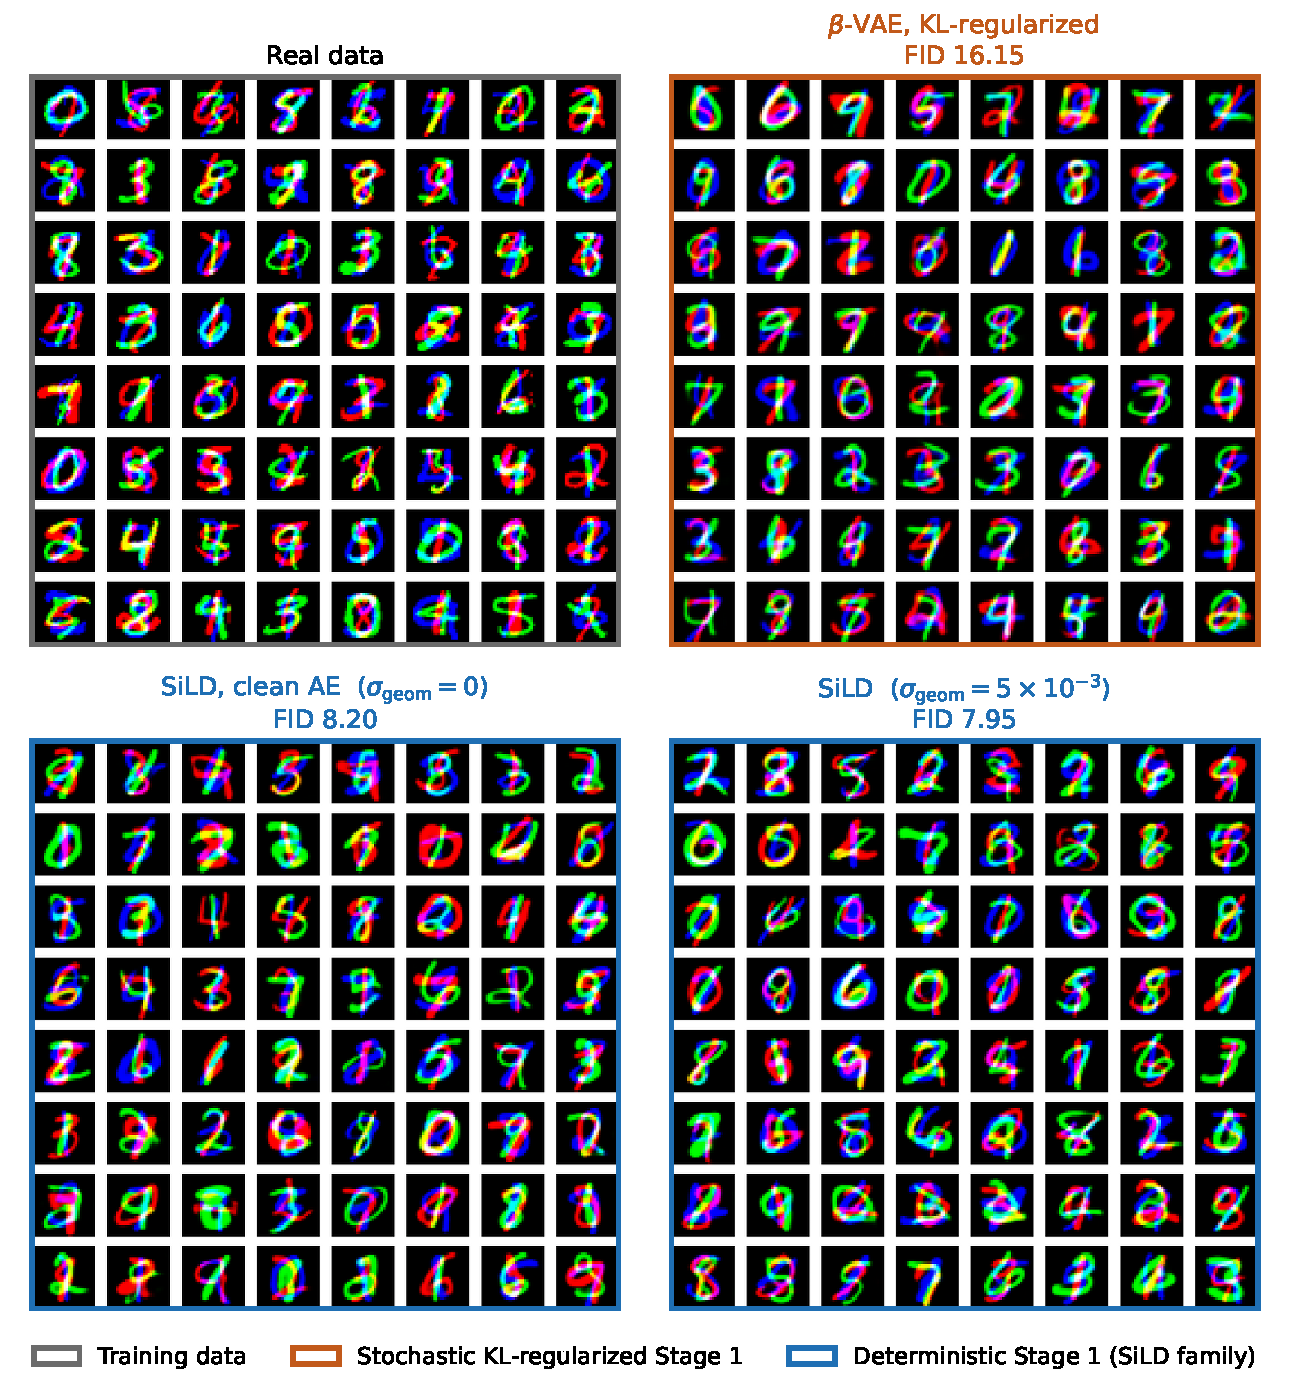
\includegraphics[width=\textwidth]{figures/stacked_mnist_stage1_family/stacked_mnist_stage1_family_seed42.pdf}
\caption{%
Uncurated Stacked MNIST samples for the three arms of
Table~\ref{tab:stacked_mnist}, plus real data (seed 42; each image is three
random MNIST digits stacked into the R/G/B channels, so there are 1000
possible modes). All panels come from runs that share the CNN backbones, the
latent score architecture, the training budget, and the Stage-2 interval
$t_2\in[0.001,0.999]$; only the Stage-1 objective differs. Every generative
arm attains full $1000/1000$ mode coverage, so none of the panels shows mode
dropping, and the qualitative differences are modest: the figure is included
to show that the clean autoencoder and SiLD are visually interchangeable
while both differ from the KL-regularized arm, which is the claim
Table~\ref{tab:stage1_noise_sweep} makes quantitatively. The remaining arms
of that table are omitted here; in particular the VP-schedule row is a
noise-form check rather than a noise-scale point and would not sit on the
same axis as the panels shown. FID values are repeated from
Table~\ref{tab:stage1_noise_sweep}.%
}
\label{fig:stacked_family_samples}
\end{figure}

\subsection{The Stage-1 objective family on molecules}
\label{app:stage1-family-mol}

Table~\ref{tab:stage1_family_mol} repeats the comparison of
Appendix~\ref{app:stage1-noise} on the molecular benchmarks. The degenerate
$\sigma\!\to\!0$ member of the family --- a clean deterministic autoencoder ---
matches SiLD on all four datasets to within $0.43$ FCD and $0.19$ percentage
points of uniqueness, with the sign of the difference inconsistent across
datasets and metrics. Each molecular cell is a single seed, so we do not
claim an ordering between the two deterministic arms; on Stacked MNIST, where
we do have three seeds, the corresponding paired difference is not
significant ($t=-0.96$). Both deterministic arms are separated from the
KL-regularized bottleneck by two orders of magnitude of uniqueness on HIV and
PCBA, and SiLD's autoencoder reaches $4.2$--$8.8\times$ lower reconstruction
error than the KL-regularized one, with the largest factor on QM9, where the
two generative models are otherwise closest.

The Stage-1 noise scale is therefore not the active ingredient; the
determinism of the Stage-1 map is. This is what the analysis predicts rather
than a weakening of it: Stage~1 is charged with identifying the
tangent--normal split, and the small-noise regime is a plateau on which any
deterministic map whose bottleneck recovers the same subspace will serve.
What the analysis does exclude is an isotropic \emph{stochastic} bottleneck,
which injects variance in the normal directions that Stage~1 is supposed to
contract; Appendix~\ref{app:collapse} shows that this is exactly how the
KL-regularized arm fails.

\begin{table}[h]
\centering
\caption{%
The Stage-1 objective family on molecules, at a common Stage-2 interval
$t_2\in[0.001,0.999]$ for all three arms (10K samples, seed 42, SELFIES;
validity is $100\%$ throughout). Encoder, decoder, and latent score network
are identical across rows; only the Stage-1 objective differs.
$\sigma\!\to\!0$ denotes the degenerate member of the family: an ordinary
clean deterministic autoencoder, with no input corruption and no KL term.
This family comparison needs its own Stage-2 interval because the paired rule
$t_2\in[t_0,0.999]$ used in Table~\ref{tab:main_results} degenerates at
$t_0=0$, so all arms are instead fixed at $t_{\min}=0.001$; the SiLD and
KL-regularized numbers therefore differ in the third digit from
Table~\ref{tab:main_results}. Bold marks the numerically best value per
dataset and metric, but every cell is a single seed and the two deterministic
arms trade wins at a margin we do not treat as meaningful.%
}
\label{tab:stage1_family_mol}
\resizebox{\textwidth}{!}{%
\begin{tabular}{llcccccc}
\toprule
\textbf{Dataset} & \textbf{Stage-1 objective}
& \textbf{Recon MSE$\downarrow$} & \textbf{Uniq.$\uparrow$}
& \textbf{Novelty$\uparrow$} & \textbf{Int.\ Div.$\uparrow$}
& \textbf{QED$\uparrow$} & \textbf{FCD$\downarrow$} \\
\midrule
\multirow{4}{*}{\textbf{QM9}}
 & Real data                               & --                      & 96.18\% & 0.0\%   & 0.919 & 0.466 & 5.05 \\
\cmidrule{2-8}
 & $\beta$-VAE, KL-regularized (LDM)       & $1.31\!\times\!10^{-3}$ & 96.94\% & 37.59\% & 0.915 & 0.473 & \textbf{4.30} \\
 & \textbf{SiLD} ($\sigma\!\to\!0$; clean AE) & $1.63\!\times\!10^{-4}$ & 97.43\% & 34.94\% & 0.917 & 0.471 & 4.41 \\
 & \textbf{SiLD} ($t_0=0.05$)              & $\mathbf{1.49\!\times\!10^{-4}}$ & \textbf{97.58\%} & 36.25\% & 0.917 & 0.468 & 4.39 \\
\midrule
\multirow{4}{*}{\textbf{HIV}}
 & Real data                               & --                      & 88.93\% & 0.0\%   & 0.898 & 0.513 & 3.24 \\
\cmidrule{2-8}
 & $\beta$-VAE, KL-regularized (LDM)       & $1.39\!\times\!10^{-3}$ & 0.99\%  & 100.0\% & 0.012 & 0.114 & 60.96 \\
 & \textbf{SiLD} ($\sigma\!\to\!0$; clean AE) & $3.28\!\times\!10^{-4}$ & \textbf{98.82\%} & 99.95\% & 0.904 & 0.430 & \textbf{10.29} \\
 & \textbf{SiLD} ($t_0=0.05$)              & $\mathbf{3.24\!\times\!10^{-4}}$ & 98.63\% & 99.95\% & 0.903 & 0.434 & 10.44 \\
\midrule
\multirow{4}{*}{\textbf{MUV}}
 & Real data                               & --                      & 95.03\% & 0.0\%   & 0.860 & 0.675 & 4.52 \\
\cmidrule{2-8}
 & $\beta$-VAE, KL-regularized (LDM)       & $6.55\!\times\!10^{-3}$ & 95.30\% & 99.98\% & 0.812 & 0.238 & 41.20 \\
 & \textbf{SiLD} ($\sigma\!\to\!0$; clean AE) & $1.60\!\times\!10^{-3}$ & \textbf{99.45\%} & 99.96\% & 0.892 & 0.513 & 19.85 \\
 & \textbf{SiLD} ($t_0=0.05$)              & $\mathbf{1.55\!\times\!10^{-3}}$ & 99.42\% & 99.97\% & 0.891 & 0.512 & \textbf{19.42} \\
\midrule
\multirow{4}{*}{\textbf{PCBA}}
 & Real data                               & --                      & 98.91\% & 0.0\%   & 0.861 & 0.637 & 9.12 \\
\cmidrule{2-8}
 & $\beta$-VAE, KL-regularized (LDM)       & $2.34\!\times\!10^{-3}$ & 0.57\%  & 94.74\% & 0.016 & 0.090 & 77.10 \\
 & \textbf{SiLD} ($\sigma\!\to\!0$; clean AE) & $5.41\!\times\!10^{-4}$ & \textbf{98.81\%} & 99.76\% & 0.895 & 0.483 & 18.04 \\
 & \textbf{SiLD} ($t_0=0.05$)              & $\mathbf{5.33\!\times\!10^{-4}}$ & 98.63\% & 99.78\% & 0.894 & 0.486 & \textbf{17.96} \\
\bottomrule
\end{tabular}%
}
\end{table}

\subsection{Stage-2 lower time bound}
\label{app:stage2-tmin}

Table~\ref{tab:stage2_tmin} varies the Stage-2 lower time bound on the
molecular benchmarks. This ablation does \emph{not} retrain Stage~1: a single
Stage-1 checkpoint (trained at $t_0=0.05$) is reused in every row, and only
the Stage-2 score network is retrained with the stated lower bound. It
therefore isolates the Stage-2 time range, not the Stage-1 noise scale, for
which Appendix~\ref{app:stage1-noise} is the relevant experiment. FCD varies
by at most $1.34$ (MUV) and by less than $0.16$ on QM9 and HIV.

\begin{table}[h]
\centering
\caption{%
Stage-2 lower time bound $t_{\min}$ on the molecular benchmarks, with Stage~1
held fixed at a single checkpoint trained at $t_0=0.05$. 10K samples, 200
sampling steps, seed 42.%
}
\label{tab:stage2_tmin}
\small
\begin{tabular}{lcccccccc}
\toprule
& \multicolumn{2}{c}{\textbf{QM9}} & \multicolumn{2}{c}{\textbf{HIV}}
& \multicolumn{2}{c}{\textbf{MUV}} & \multicolumn{2}{c}{\textbf{PCBA}} \\
\cmidrule(lr){2-3}\cmidrule(lr){4-5}\cmidrule(lr){6-7}\cmidrule(lr){8-9}
$t_{\min}$ & Uniq. & FCD & Uniq. & FCD & Uniq. & FCD & Uniq. & FCD \\
\midrule
$0.01$ & 97.44\% & 4.32 & 98.81\% & 10.35 & 99.35\% & 19.14 & 98.64\% & 17.95 \\
$0.02$ & 97.69\% & 4.47 & 98.76\% & 10.34 & 99.35\% & 19.23 & 98.70\% & 17.89 \\
$0.05$ & 97.23\% & 4.43 & 98.68\% & 10.32 & 99.31\% & 19.35 & 98.65\% & 17.87 \\
$0.10$ & 97.21\% & 4.33 & 98.65\% & 10.51 & 99.48\% & 18.86 & 98.93\% & 17.67 \\
$0.20$ & 97.29\% & 4.44 & 98.86\% & 10.44 & 99.38\% & 18.14 & 98.94\% & 17.08 \\
\bottomrule
\end{tabular}
\end{table}

\subsection{Where the KL-regularized arm fails}
\label{app:collapse}

To locate the failure we decompose the pipeline into three decodes that share
one trained model: \textbf{(A)} \emph{round trip} --- encode real test
molecules and decode, which exercises Stage~1 alone; \textbf{(B)}
\emph{generation} --- the full reverse latent diffusion followed by decoding;
and \textbf{(C)} \emph{prior decode} --- decode samples from
$\mathcal N(0,I)$ directly, bypassing the score network. If a model's
diversity were destroyed by the latent diffusion, (A) would be healthy and
(B) degraded. Table~\ref{tab:collapse_abc} shows the opposite for the
KL-regularized arm: (A) is already collapsed, and (A), (B), and (C) agree,
so the decoder's output is nearly independent of its input.

\begin{table}[h]
\centering
\caption{%
Pipeline decomposition, 10K samples per cell, seed 42. (A) encode real
molecules and decode; (B) full latent-diffusion generation; (C) decode
$\mathcal N(0,I)$ samples directly. For the KL-regularized arm on HIV and
PCBA all three agree at near-zero uniqueness and IntDiv, identifying Stage~1
as the point of failure.%
}
\label{tab:collapse_abc}
\small
\resizebox{\textwidth}{!}{%
\begin{tabular}{llccccccc}
\toprule
& & \multicolumn{3}{c}{\textbf{(A) round trip}} & \multicolumn{2}{c}{\textbf{(B) generation}} & \multicolumn{2}{c}{\textbf{(C) prior decode}} \\
\cmidrule(lr){3-5}\cmidrule(lr){6-7}\cmidrule(lr){8-9}
\textbf{Dataset} & \textbf{Stage-1 objective} & Uniq. & Int.\ Div. & FCD & Uniq. & FCD & Uniq. & FCD \\
\midrule
\multirow{2}{*}{\textbf{QM9}}
 & $\beta$-VAE, KL-regularized & 100.0\% & 0.917 & 6.09 & 99.61\% & 4.72 & 100.0\% & 5.72 \\
 & \textbf{SiLD}               & 100.0\% & 0.919 & 5.94 & 100.0\% & 5.10 & 98.05\% & 8.68 \\
\midrule
\multirow{2}{*}{\textbf{HIV}}
 & $\beta$-VAE, KL-regularized & 0.95\%  & 0.019 & 60.95 & 0.98\%  & 60.91 & 0.93\%  & 61.17 \\
 & \textbf{SiLD}               & 87.76\% & 0.902 & 5.09  & 98.84\% & 10.40 & 93.97\% & 17.67 \\
\midrule
\multirow{2}{*}{\textbf{PCBA}}
 & $\beta$-VAE, KL-regularized & 0.53\%  & 0.020 & 77.10 & 0.58\%  & 77.12 & 0.65\%  & 77.06 \\
 & \textbf{SiLD}               & 97.79\% & 0.885 & 11.03 & 98.72\% & 18.04 & 92.13\% & 28.63 \\
\bottomrule
\end{tabular}%
}
\end{table}

Table~\ref{tab:collapse_latent} gives the mechanism. On the raw encoder
output, the KL-regularized arm has driven $99.6\%$ (HIV) and $92.6\%$ (PCBA)
of coordinates to standard deviation below $10^{-3}$, with a
largest-to-smallest ratio in the thousands; SiLD has no such coordinate and a
ratio below $5$. On QM9 --- the one dataset where the two methods are
comparable --- the KL arm has no collapsed coordinates either, which is
consistent with the claim that posterior collapse, not KL regularization per
se, is what the two-stage separation avoids. The effective ranks in the last
three columns are computed after per-coordinate standardization, so they
measure the dimension of the occupied support rather than collapse; in every
arm the generated support matches the real support closely, while the
Gaussian prior occupies a far larger subspace.

\begin{table}[h]
\centering
\caption{%
Latent statistics, 10K encodings, seed 42. Dead coordinates and the
standard-deviation ratio (largest over smallest, and ``dead'' meaning
standard deviation below $10^{-3}$) are computed on the \emph{raw} encoder
output; effective rank (participation ratio) is computed after
per-coordinate standardization, on real encodings ($z_{\mathrm{real}}$), on
latents produced by Stage~2 ($z_{\mathrm{gen}}$), and on prior samples
($z_{\mathrm{prior}}$).%
}
\label{tab:collapse_latent}
\small
\resizebox{\textwidth}{!}{%
\begin{tabular}{llcccccc}
\toprule
\textbf{Dataset} & \textbf{Stage-1 objective} & $d_z$
& dead coords & std ratio
& eff.\ rank $z_{\mathrm{real}}$ & eff.\ rank $z_{\mathrm{gen}}$
& eff.\ rank $z_{\mathrm{prior}}$ \\
\midrule
\multirow{2}{*}{\textbf{QM9}}
 & $\beta$-VAE, KL-regularized & 128 & 0.0\%   & 80.4   & 3.10  & 3.42  & 84.9 \\
 & \textbf{SiLD}               & 128 & 0.0\%   & 2.0    & 25.08 & 26.84 & 85.8 \\
\midrule
\multirow{2}{*}{\textbf{HIV}}
 & $\beta$-VAE, KL-regularized & 512 & 99.6\%  & 2739.2 & 17.84 & 11.43 & 453.6 \\
 & \textbf{SiLD}               & 512 & 0.0\%   & 4.6    & 8.68  & 8.07  & 454.1 \\
\midrule
\multirow{2}{*}{\textbf{PCBA}}
 & $\beta$-VAE, KL-regularized & 256 & 92.6\%  & 1753.5 & 16.86 & 16.12 & 240.6 \\
 & \textbf{SiLD}               & 256 & 0.0\%   & 3.5    & 7.91  & 7.73  & 240.4 \\
\bottomrule
\end{tabular}%
}
\end{table}

In the SiLD latents the generated and real supports agree in effective rank
(participation ratio $8.07$ vs.\ $8.68$ out of $512$ on HIV, $7.73$ vs.\
$7.91$ out of $256$ on PCBA) while the Gaussian prior occupies $454$ and
$240$ respectively, so Stage~2 reproduces a support of the same low dimension
as the data rather than filling the latent cube.
Appendix~\ref{app:celeba-boundary} marks where the
deterministic-versus-KL ordering stops holding.

\subsection{Sampling-step budget}
\label{app:steps}

Table~\ref{tab:steps_sweep} varies the number of reverse-diffusion steps at
sampling time with the trained model held fixed. Quality is essentially flat
from $25$ to $500$ steps on all four molecular benchmarks: the FCD spread is
$0.30$ (QM9), $0.35$ (HIV), $0.97$ (MUV), and $0.68$ (PCBA), and the cheapest
setting is not systematically the worst. Generating 10K molecules takes
$1.3$--$1.7$\,s at $25$ steps against $21.6$--$22.3$\,s at $500$.

\begin{table}[h]
\centering
\caption{%
Reverse-diffusion step count at sampling time, with the trained SiLD model
held fixed. 10K samples, seed 42; wall-clock is the sampling time for the
full 10K batch on one GPU.%
}
\label{tab:steps_sweep}
\small
\begin{tabular}{lcccccccccc}
\toprule
& \multicolumn{2}{c}{\textbf{QM9}} & \multicolumn{2}{c}{\textbf{HIV}}
& \multicolumn{2}{c}{\textbf{MUV}} & \multicolumn{2}{c}{\textbf{PCBA}}
& \multicolumn{2}{c}{\textbf{wall-clock (s)}} \\
\cmidrule(lr){2-3}\cmidrule(lr){4-5}\cmidrule(lr){6-7}\cmidrule(lr){8-9}\cmidrule(lr){10-11}
steps & Uniq. & FCD & Uniq. & FCD & Uniq. & FCD & Uniq. & FCD & min & max \\
\midrule
$25$  & 97.44\% & 4.14 & 98.58\% & 10.81 & 99.53\% & 20.30 & 98.47\% & 18.44 & 1.3 & 1.7 \\
$50$  & 97.77\% & 4.27 & 98.69\% & 10.51 & 99.41\% & 19.73 & 98.59\% & 17.94 & 2.2 & 2.6 \\
$100$ & 97.36\% & 4.22 & 98.79\% & 10.49 & 99.24\% & 19.52 & 98.76\% & 17.76 & 4.3 & 4.8 \\
$200$ & 97.65\% & 4.38 & 98.78\% & 10.46 & 99.33\% & 19.33 & 98.67\% & 17.83 & 8.7 & 9.1 \\
$500$ & 97.73\% & 4.44 & 98.77\% & 10.49 & 99.44\% & 19.50 & 98.74\% & 17.99 & 21.6 & 22.3 \\
\bottomrule
\end{tabular}
\end{table}

\subsection{Novelty--fidelity trade-off on QM9}
\label{app:novelty-tradeoff}

QM9 is the one benchmark on which SiLD does not improve novelty over the
KL-regularized baseline (Table~\ref{tab:main_results}). The dataset is small
and nearly exhaustively enumerated, so novelty and distributional fidelity
are in direct tension there, and both are reachable from the same trained
model by rescaling the initial latent noise or the score at sampling time.
Table~\ref{tab:novelty_tradeoff} traces that frontier: inflating the initial
noise from $\sigma_{\mathrm{init}}=1.0$ to $1.3$ raises novelty from $35.8\%$
to $51.7\%$ and uniqueness from $97.5\%$ to $98.4\%$ while FCD degrades only
from $4.22$ to $5.19$; pushing further, or raising the score temperature,
buys novelty up to $97.7\%$ at a clear cost in FCD and QED. We report the
untuned $\sigma_{\mathrm{init}}=1.0$ setting everywhere in the main text.

\begin{table}[h]
\centering
\caption{%
Sampling-time novelty--fidelity trade-off on QM9, from a single trained SiLD
model (10K samples, 50 steps, seed 42). $\sigma_{\mathrm{init}}$ scales the
initial latent noise; $T$ scales the predicted score. The first row is the
setting used in the main text.%
}
\label{tab:novelty_tradeoff}
\small
\begin{tabular}{llccccc}
\toprule
$\sigma_{\mathrm{init}}$ & $T$ & Uniq.$\uparrow$ & Novelty$\uparrow$ & Int.\ Div.$\uparrow$ & QED$\uparrow$ & FCD$\downarrow$ \\
\midrule
$1.0$ & $1.0$ & 97.51\% & 35.8\% & 0.917 & 0.470 & 4.22 \\
$1.1$ & $1.0$ & 97.91\% & 42.0\% & 0.921 & 0.465 & 4.56 \\
$1.2$ & $1.0$ & 98.12\% & 46.5\% & 0.924 & 0.461 & 4.99 \\
$1.3$ & $1.0$ & 98.44\% & 51.7\% & 0.925 & 0.457 & 5.19 \\
$1.5$ & $1.0$ & 98.50\% & 61.3\% & 0.930 & 0.448 & 5.90 \\
$2.0$ & $1.0$ & 97.87\% & 80.7\% & 0.937 & 0.419 & 6.66 \\
\midrule
$1.0$ & $1.1$ & 98.47\% & 62.0\% & 0.928 & 0.448 & 5.43 \\
$1.0$ & $1.2$ & 97.76\% & 82.8\% & 0.937 & 0.418 & 6.20 \\
$1.0$ & $1.3$ & 91.45\% & 94.6\% & 0.944 & 0.366 & 7.94 \\
$1.0$ & $1.5$ & 86.37\% & 97.7\% & 0.946 & 0.324 & 9.61 \\
\midrule
$1.2$ & $1.2$ & 94.61\% & 91.8\% & 0.942 & 0.388 & 7.19 \\
$1.3$ & $1.2$ & 91.49\% & 94.4\% & 0.943 & 0.370 & 7.87 \\
$1.5$ & $1.3$ & 87.02\% & 97.8\% & 0.947 & 0.324 & 9.77 \\
\bottomrule
\end{tabular}
\end{table}

\subsection{Boundary of the deterministic-versus-KL ordering}
\label{app:celeba-boundary}

The ordering between deterministic and KL-regularized Stage-1 objectives is
not universal, and Table~\ref{tab:celeba_boundary} marks where it reverses.
On CelebA at $64\times64$ with a small KL weight ($10^{-4}$) and no auxiliary
regularizer, the KL-regularized arm attains the best FID and the best
reconstruction, and the pure deterministic autoencoder is worst. The latent
MMD to a standard Gaussian explains the reversal: the KL term is doing its
intended job of matching the prior ($0.0078$ against $0.0150$ for both
deterministic arms), and on this dataset it does so without collapsing any
coordinate --- exactly the regime in which Appendix~\ref{app:collapse}
predicts that removing KL buys nothing. Recovering the ordering on CelebA
requires an auxiliary prior-matching term in place of KL, which is what the
MMD- and GAN-regularized variants in the main text supply.

\begin{table}[h]
\centering
\caption{%
CelebA ($64\times64$), seed 42, identical encoder, decoder, and score network;
FID on 2048 samples, 500 sampling steps, $20$K Stage-1 and $60$K Stage-2
steps. ``Latent MMD'' is the maximum mean discrepancy between the encoded
data and $\mathcal N(0,I)$. No auxiliary regularizer (MMD, GAN, LPIPS) is
active in any row.%
}
\label{tab:celeba_boundary}
\small
\begin{tabular}{lcccc}
\toprule
Stage-1 objective & Recon MSE $\downarrow$ & Latent MMD $\downarrow$ & $\epsilon$-loss $\downarrow$ & FID $\downarrow$ \\
\midrule
$\beta$-VAE, KL-regularized ($\lambda_{\mathrm{KL}}=10^{-4}$) & $\mathbf{1.283\!\times\!10^{-3}}$ & $\mathbf{0.0078}$ & $\mathbf{0.277}$ & $\mathbf{63.64}$ \\
SiLD ($\sigma_{\mathrm{geom}}=5\!\times\!10^{-3}$)            & $1.338\!\times\!10^{-3}$ & $0.0150$ & $0.315$ & $64.70$ \\
SiLD, clean AE ($\sigma_{\mathrm{geom}}=0$)                   & $1.449\!\times\!10^{-3}$ & $0.0151$ & $0.318$ & $66.06$ \\
\bottomrule
\end{tabular}
\end{table}

% ---------------------------------------------------------------------
% OPEN ITEM: the subsection below reports a result that is unfavourable to
% SiLD. It is drafted so it is ready to use, but whether to include it is a
% judgement call that has not been made yet. Delete the subsection if not.
% ---------------------------------------------------------------------
\subsection{Equivariant 3D molecular latents: a negative result}
\label{app:3d}

The two-stage separation does not help when the latent already carries a
strong geometric inductive bias. Substituting the SiLD Stage-1 objective into
the E(3)-equivariant autoencoder of GeoLDM~\cite{xu2023geometric} on QM9 with
3D coordinates, and training both arms identically, leaves SiLD behind the
KL-regularized original on every stability and validity metric
(Table~\ref{tab:qm9_3d}). We report this rather than omitting it: the
mechanism identified in Appendix~\ref{app:collapse} is posterior collapse in
a generic bottleneck, and an equivariant encoder whose latent is tied to
atom-wise geometry does not exhibit it, so the premise for the improvement is
absent. Both arms also remain far below the published GeoLDM numbers under
our reduced training budget, so the comparison should be read as a matched
ablation and not as a reproduction.

\begin{table}[h]
\centering
\caption{%
QM9 with 3D coordinates, E(3)-equivariant GeoLDM backbone, 10K samples.
Both arms in the upper block come from one paired run with identical
budgets; the last row is a separately trained KL-regularized arm. Atom and
molecule stability follow the standard valency-based definitions.%
}
\label{tab:qm9_3d}
\small
\begin{tabular}{lcccc}
\toprule
Stage-1 objective & Atom stab.$\uparrow$ & Mol.\ stab.$\uparrow$ & Validity$\uparrow$ & Valid \& unique$\uparrow$ \\
\midrule
Real data                                & 95.13\% & 93.92\% & 95.28\% & 91.55\% \\
\midrule
$\beta$-VAE, KL-regularized (GeoLDM)     & \textbf{45.80\%} & \textbf{38.09\%} & \textbf{47.52\%} & \textbf{47.41\%} \\
SiLD Stage-1 in the GeoLDM latent        & 42.94\% & 32.89\% & 44.65\% & 44.61\% \\
\midrule
$\beta$-VAE, KL-regularized (separate run) & 49.11\% & 45.14\% & 50.20\% & 49.88\% \\
\bottomrule
\end{tabular}
\end{table}
